\label{optimization_EM}

In this chapter, we will be in the Target side, trying  to find an optimized escaping maneuver from the Attacker. We will use two optimization techniques, \textit{Monte Carlo} and \textit{Genetic algorithm}.


\section{Models \& Simulations}
% ===================================================

In this section we will simulate equations in sec. \ref{PNeqations} for proportional navigation using MATLAB and Simulink.



\subsection{Simulation for some target maneuver cases [using MATLAB]}
In this subsection we will use MATLAB to simulate the equations in Sec. \ref{PNeqations} for proportional navigation. We will solve the initial value problem of differential equations using second-order Runge-Kutta numerical integration technique, then we will draw the trajectories of the pursuit and evasion for 4 cases for the Target maneuver error source, and we will deduce the effect of the effective navigation ratio $N'$ and the other type of the error source; Heading error. 
\subsubsection{Zero Target maneuver}
In this case the evader (Target - plane) does not do any effort to escape, it just moves in a straight line, as we see in Fig. \ref{trajectoryXNT0HE0N4}. So the pursuer (Attacker - Missile) does not have to bleed much energy to reach the Target.

In the case of \textbf{zero Heading error} the effective navigation ratio has no effect on the simulation engagement at all. The missile's acceleration will be zero as in Fig. \ref{missile accelerationXNT0HE0N4}.

\begin{figure}[H]
	\centering
	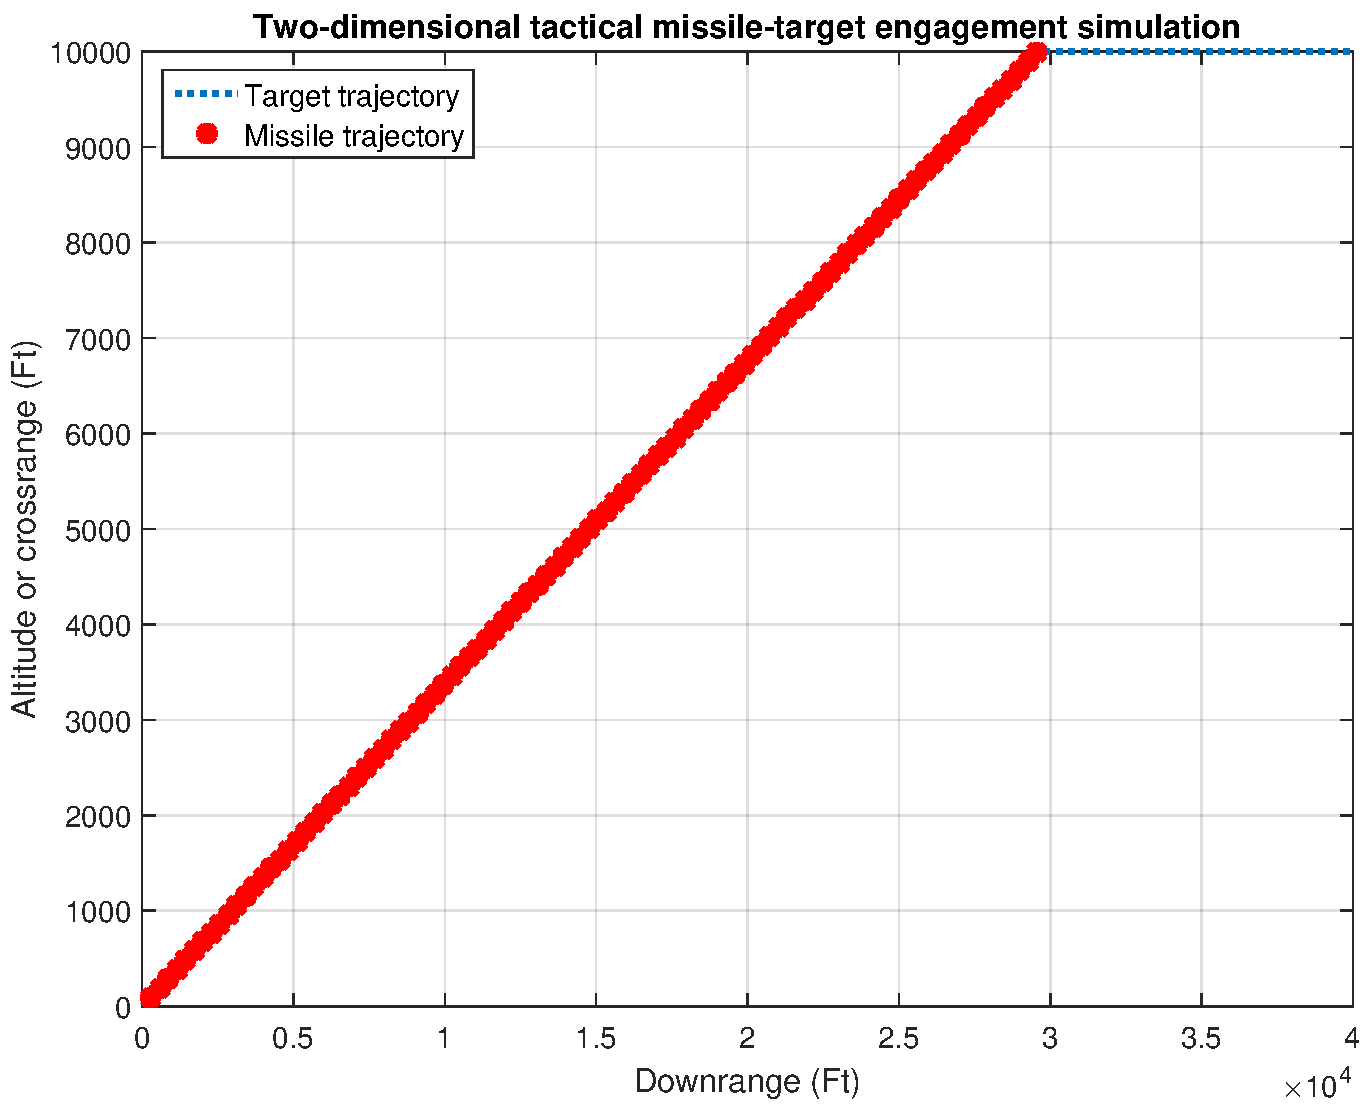
\includegraphics[scale = 0.35]{fig/trajectoryXNT0HE0N4.pdf}
	\caption{Trajectory of the target and attacker in case of zero target maneuver with zero heading error and $N'=4$.}
	\label{trajectoryXNT0HE0N4}
\end{figure}


\begin{figure}[H]
	\centering
	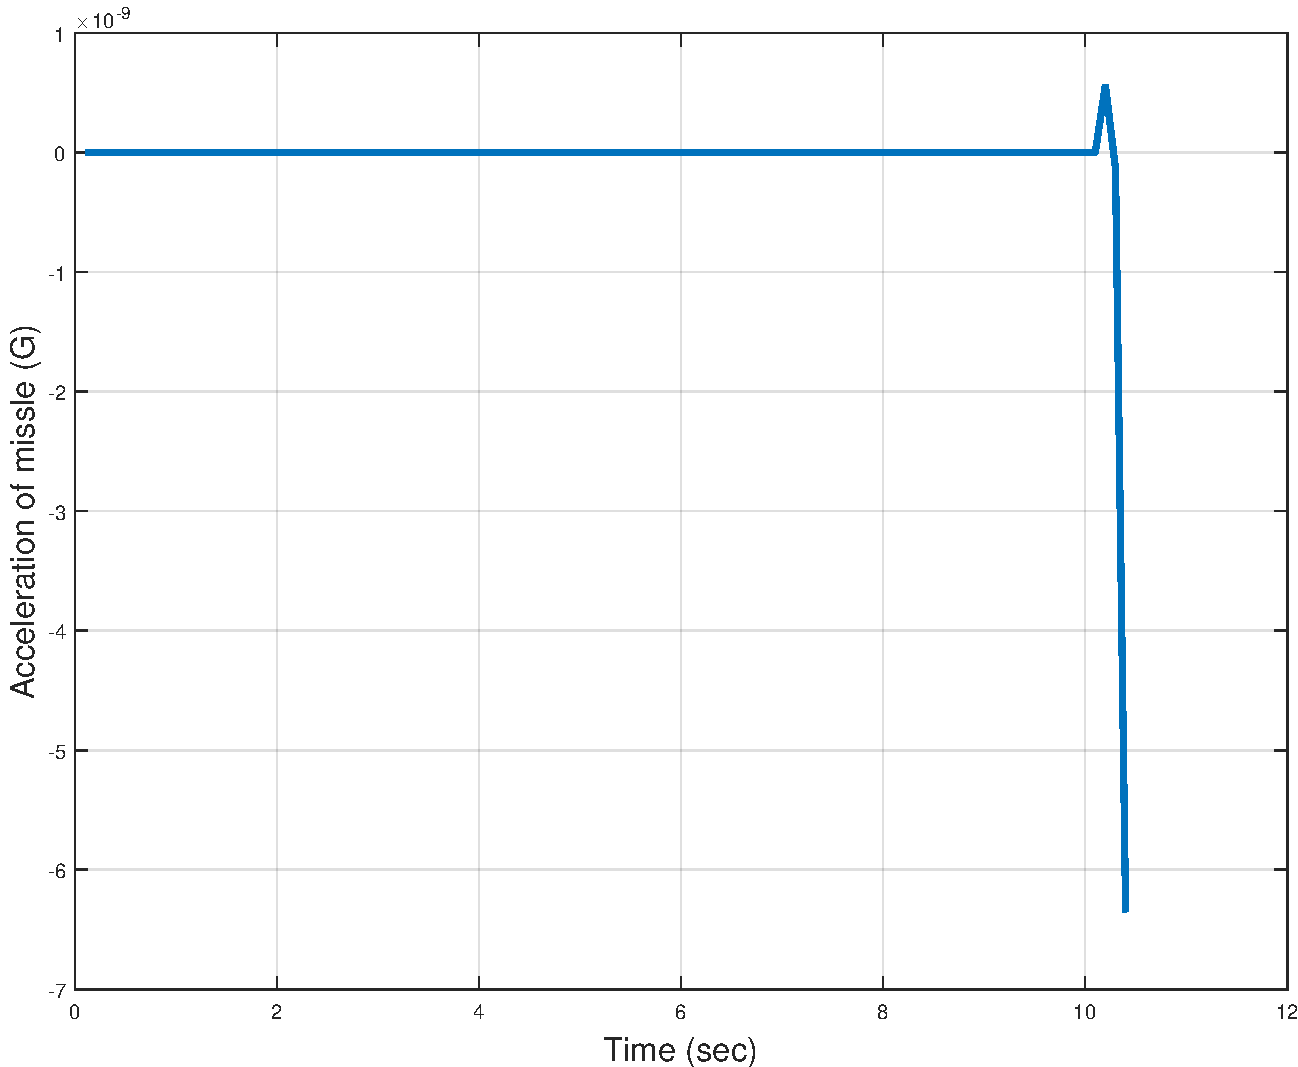
\includegraphics[scale = 0.58]{fig/MissileAccelerationXNT0HE0N4.pdf}
	\caption{Missile acceleration in case of zero target maneuver with zero heading error and $N'=4$ .}
	\label{missile accelerationXNT0HE0N4}
\end{figure}


\begin{figure}[H]
	\centering
	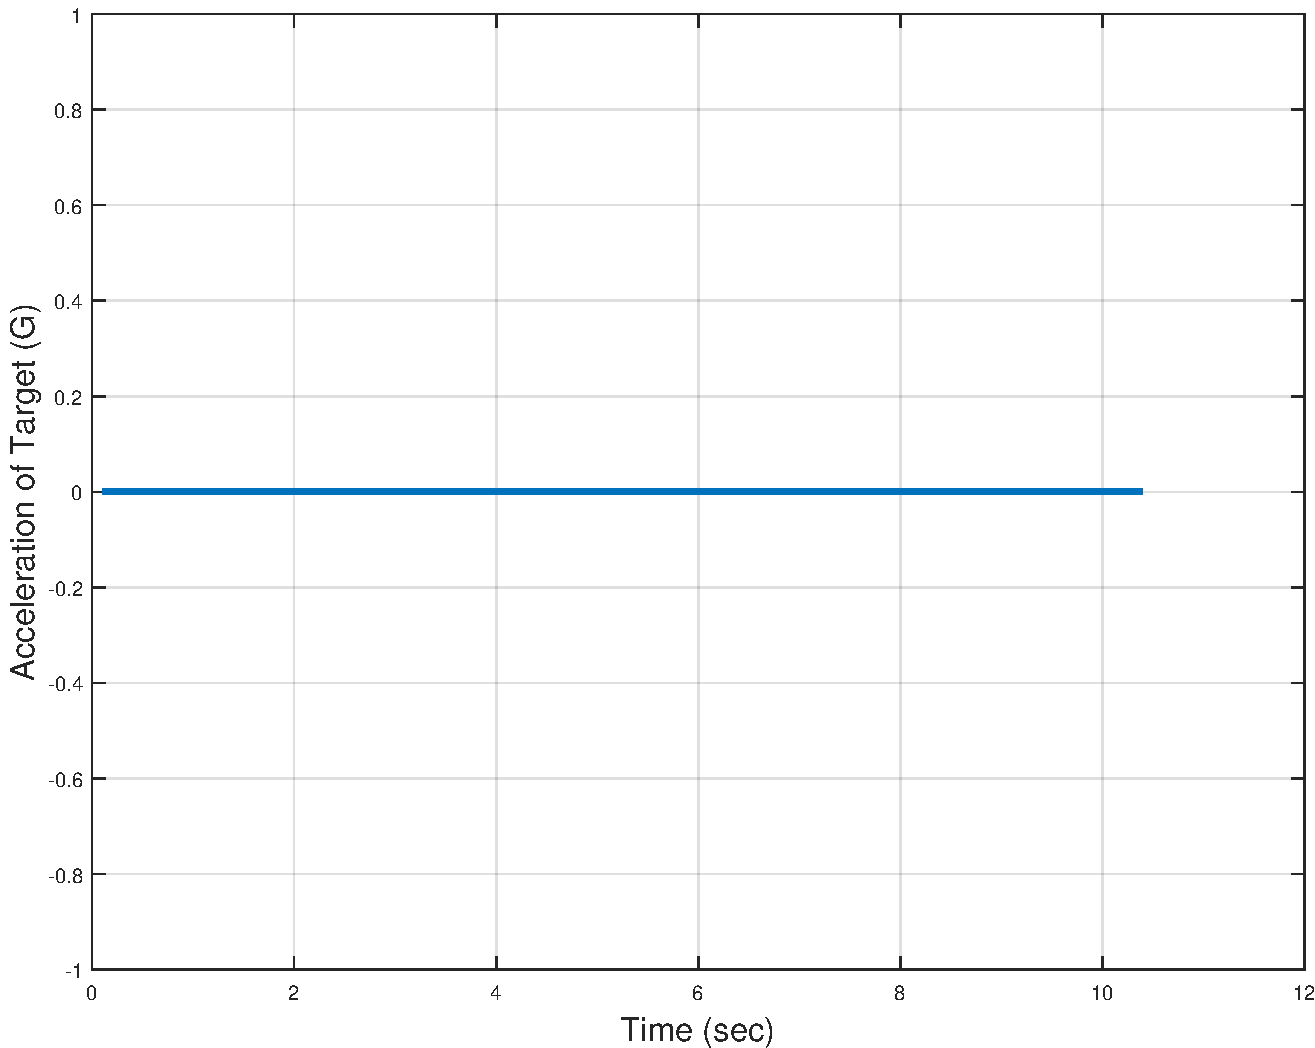
\includegraphics[scale = 0.58]{fig/TargetAccelerationXNT0HE0N4.pdf}
	\caption{Target acceleration in case of zero target maneuver with zero heading error and $N'=4$ .}
	\label{Target accelerationXNT0HE0N4}
\end{figure}


In the case of \textbf{Heading error = -20} increasing the effective navigation ratio causes heading error to be removed rapidly as we see from  Fig. \ref{trajectory20N3}, Fig. \ref{trajectory20N4} and Fig. \ref{trajectory20N5}. The effective navigation ratio has an effect on the acceleration of the missile; the way that the missile will bleed energy as we see from Fig. \ref{missile acceleration20N3} , Fig. \ref{missile acceleration20N4} and Fig. \ref{missile acceleration20N5}. The total acceleration (area under the curve) is increasingly inversely proportional with the effective navigation ratio $N'$ .


\begin{figure}[H]
	\centering
	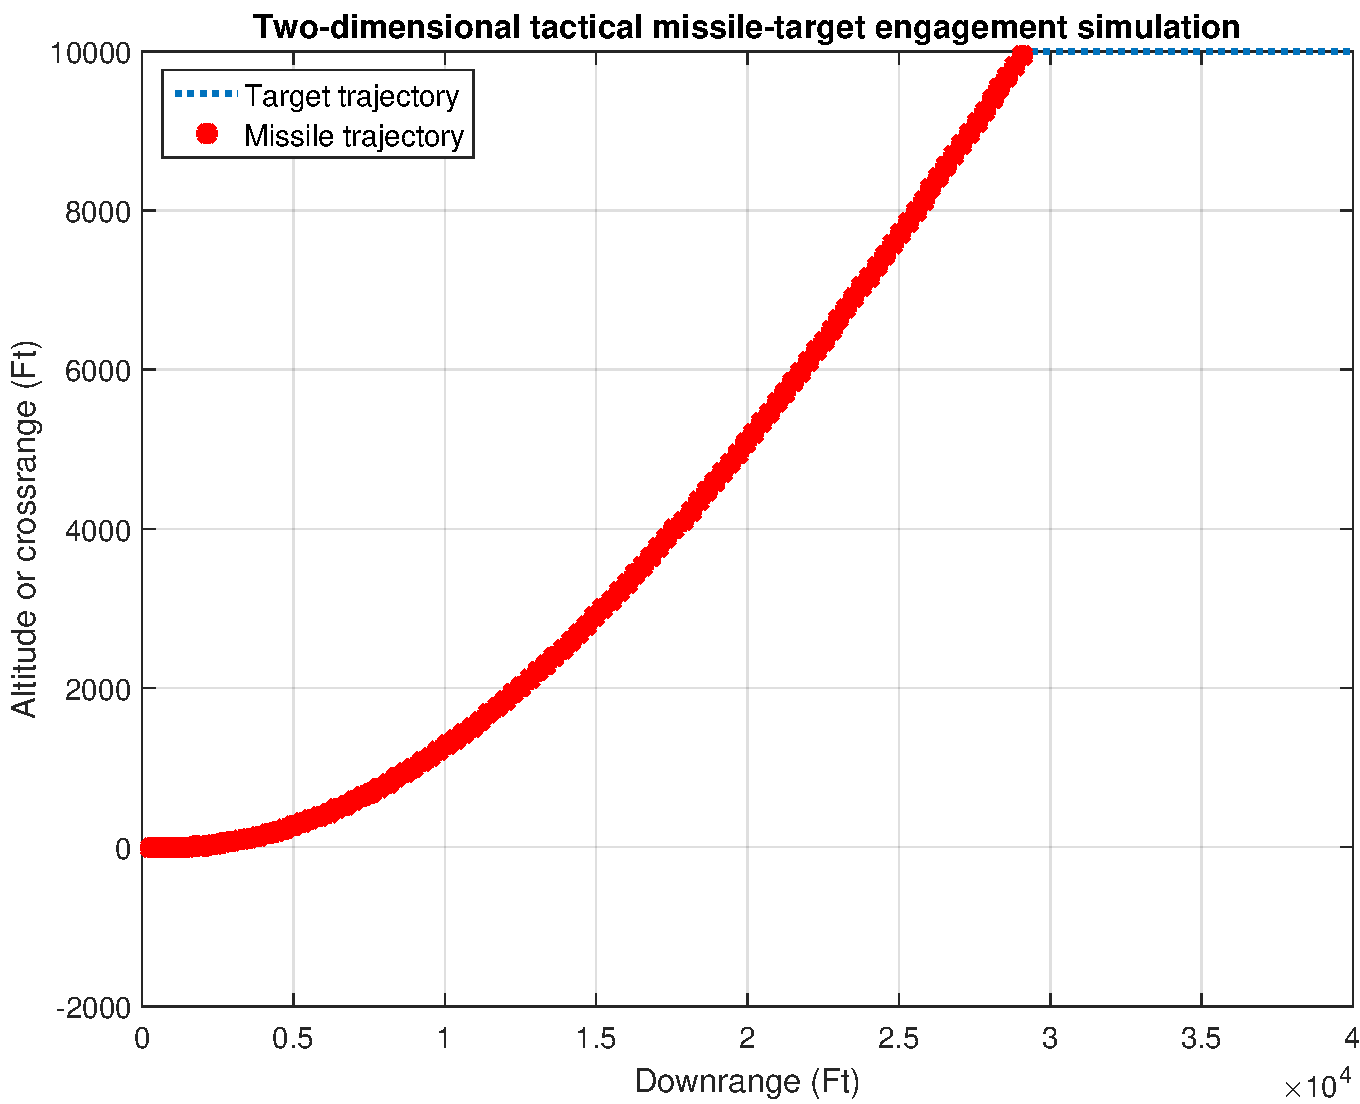
\includegraphics[scale = 0.48]{fig/trajectoryXNT0HE20N3.pdf}
	\caption{Trajectory of the target and attacker in case of zero target maneuver with heading error=-20 and $N'=3$.}
	\label{trajectory20N3}
\end{figure}

\begin{figure}[H]
	\centering
	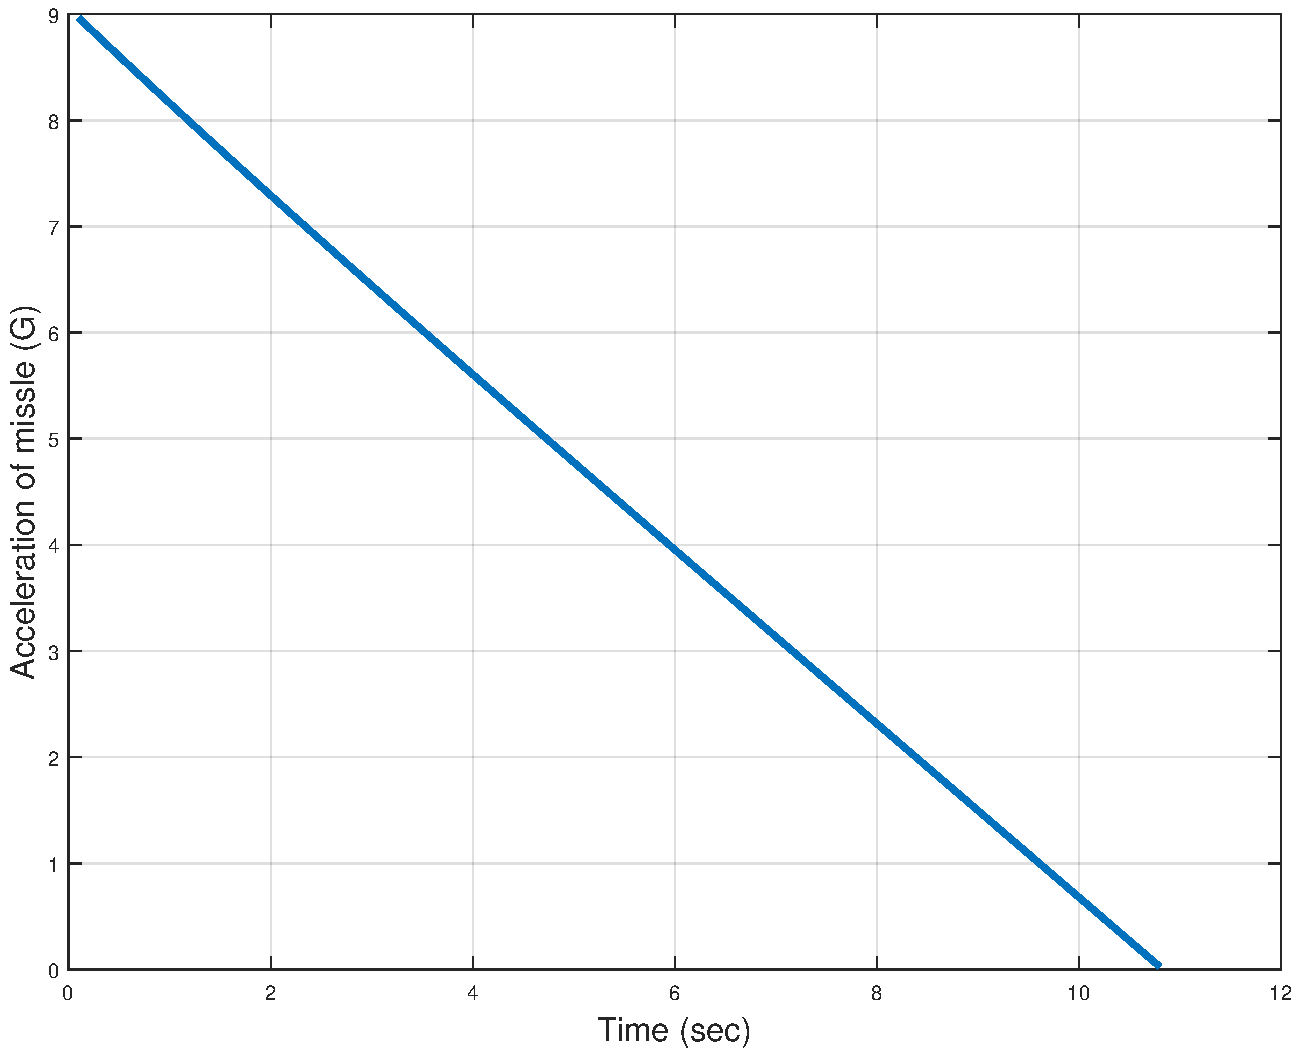
\includegraphics[scale = 0.48]{fig/MissileAccelerationXNT0HE20N3.pdf}
	\caption{Missile acceleration in case of zero target maneuver with heading error=-20 and $N'=3$ .}
	\label{missile acceleration20N3}
\end{figure}


\begin{figure}[H]
	\centering
	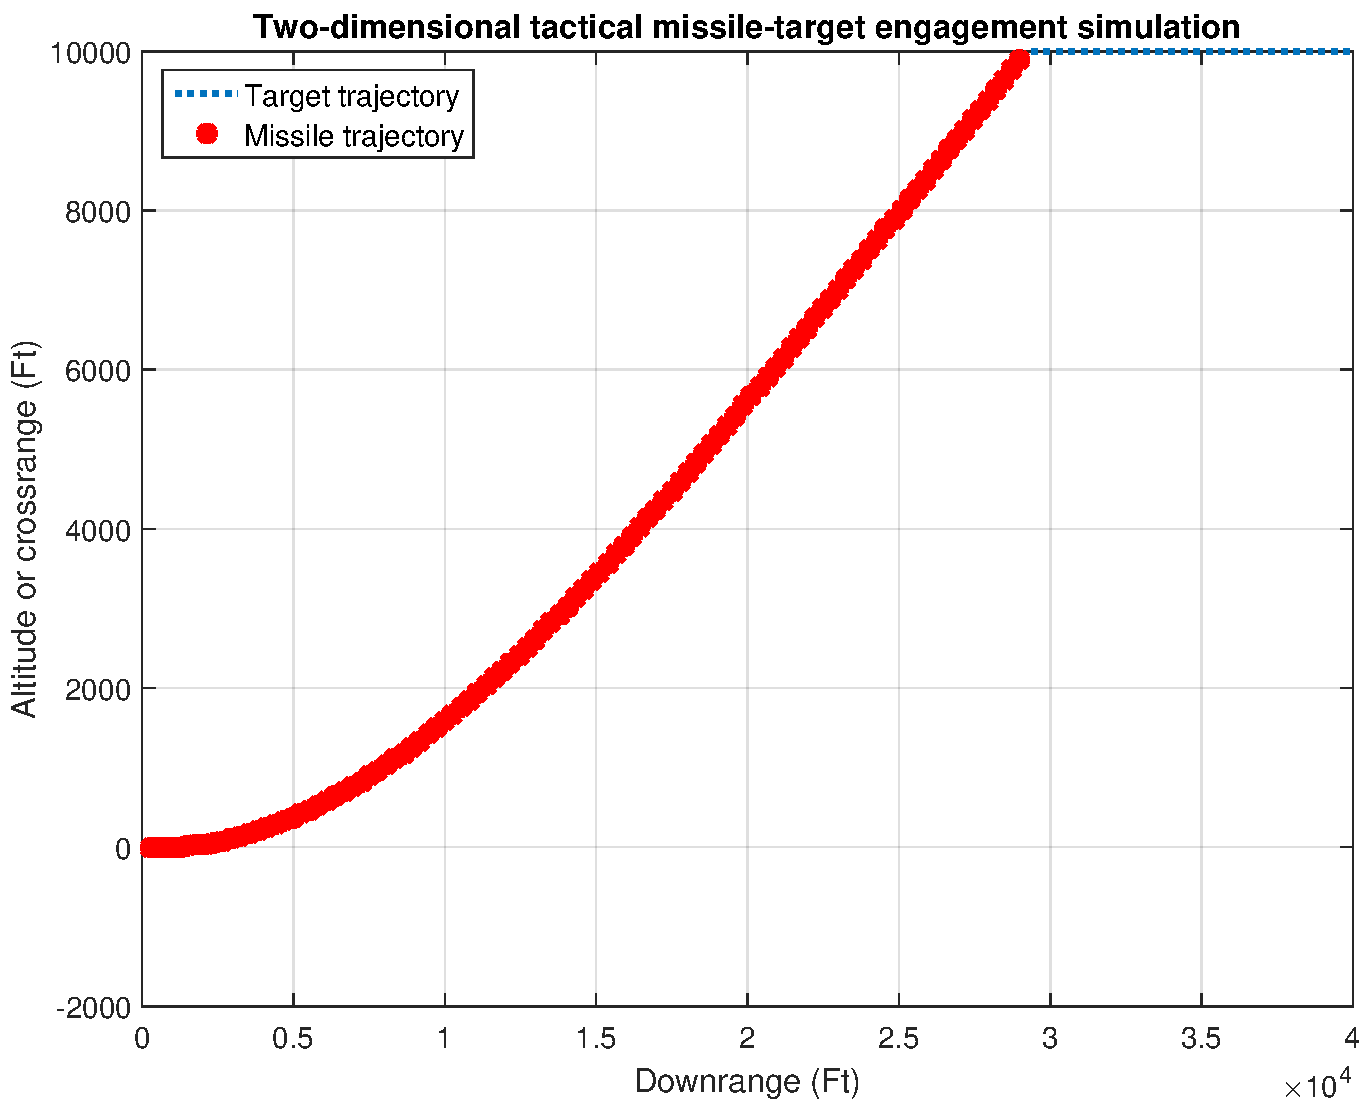
\includegraphics[scale = 0.57]{fig/trajectoryXNT0HE20N4.pdf}
	\caption{Trajectory of the target and attacker in case of zero target maneuver with heading error=-20 and $N'=4$.}
	\label{trajectory20N4}
\end{figure}


\begin{figure}[H]
	\centering
	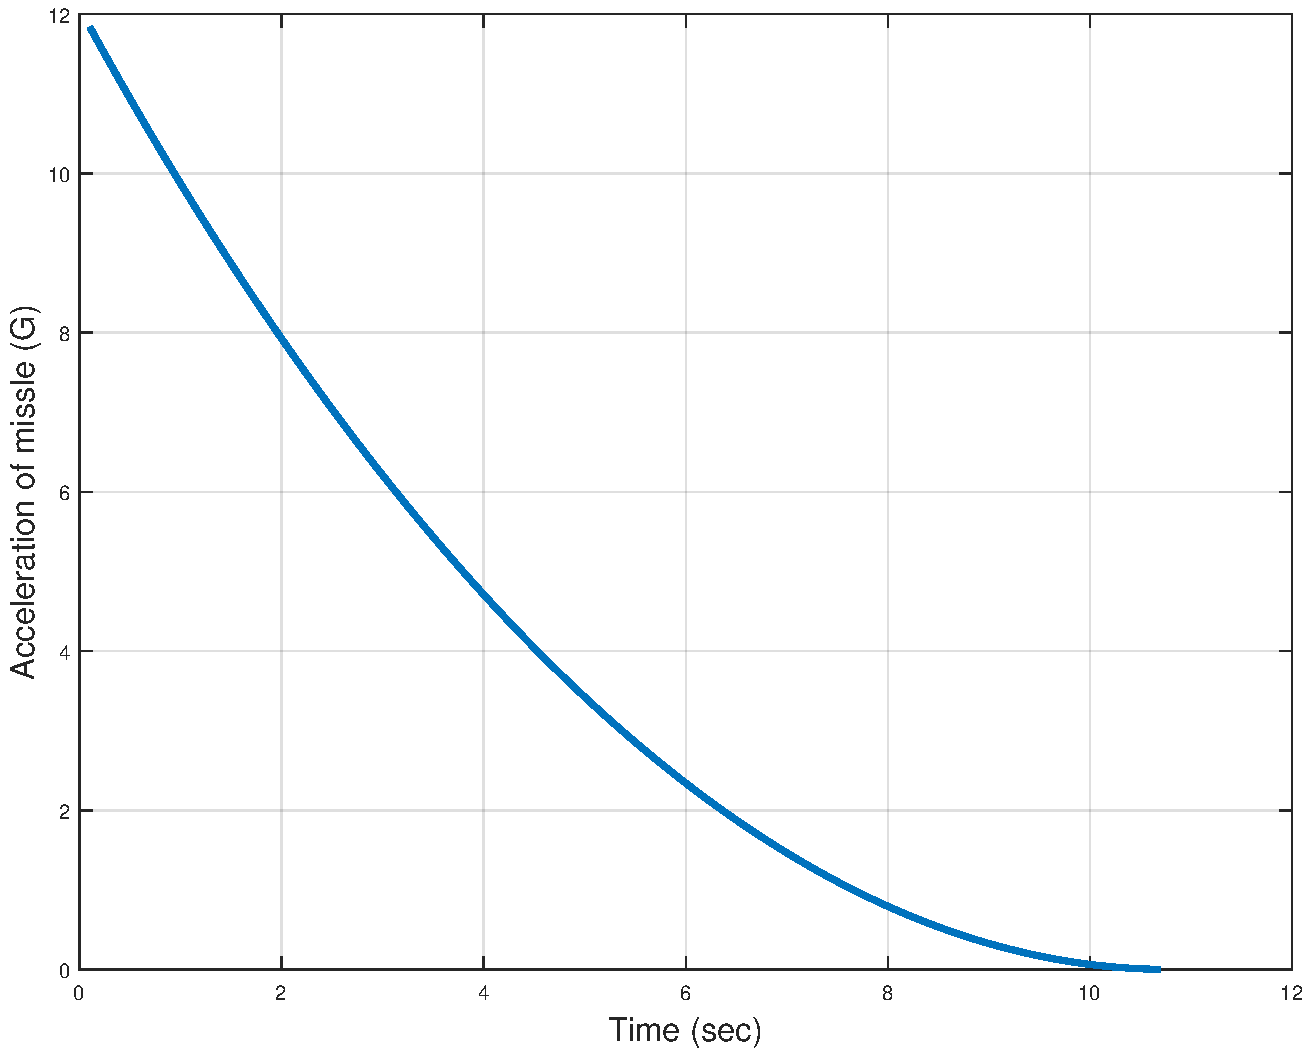
\includegraphics[scale = 0.57]{fig/MissileAccelerationXNT0HE20N4.pdf}
	\caption{Missile acceleration in case of zero target maneuver with heading error=-20 and $N'=4$ .}
	\label{missile acceleration20N4}
\end{figure}


\begin{figure}[H]
	\centering
	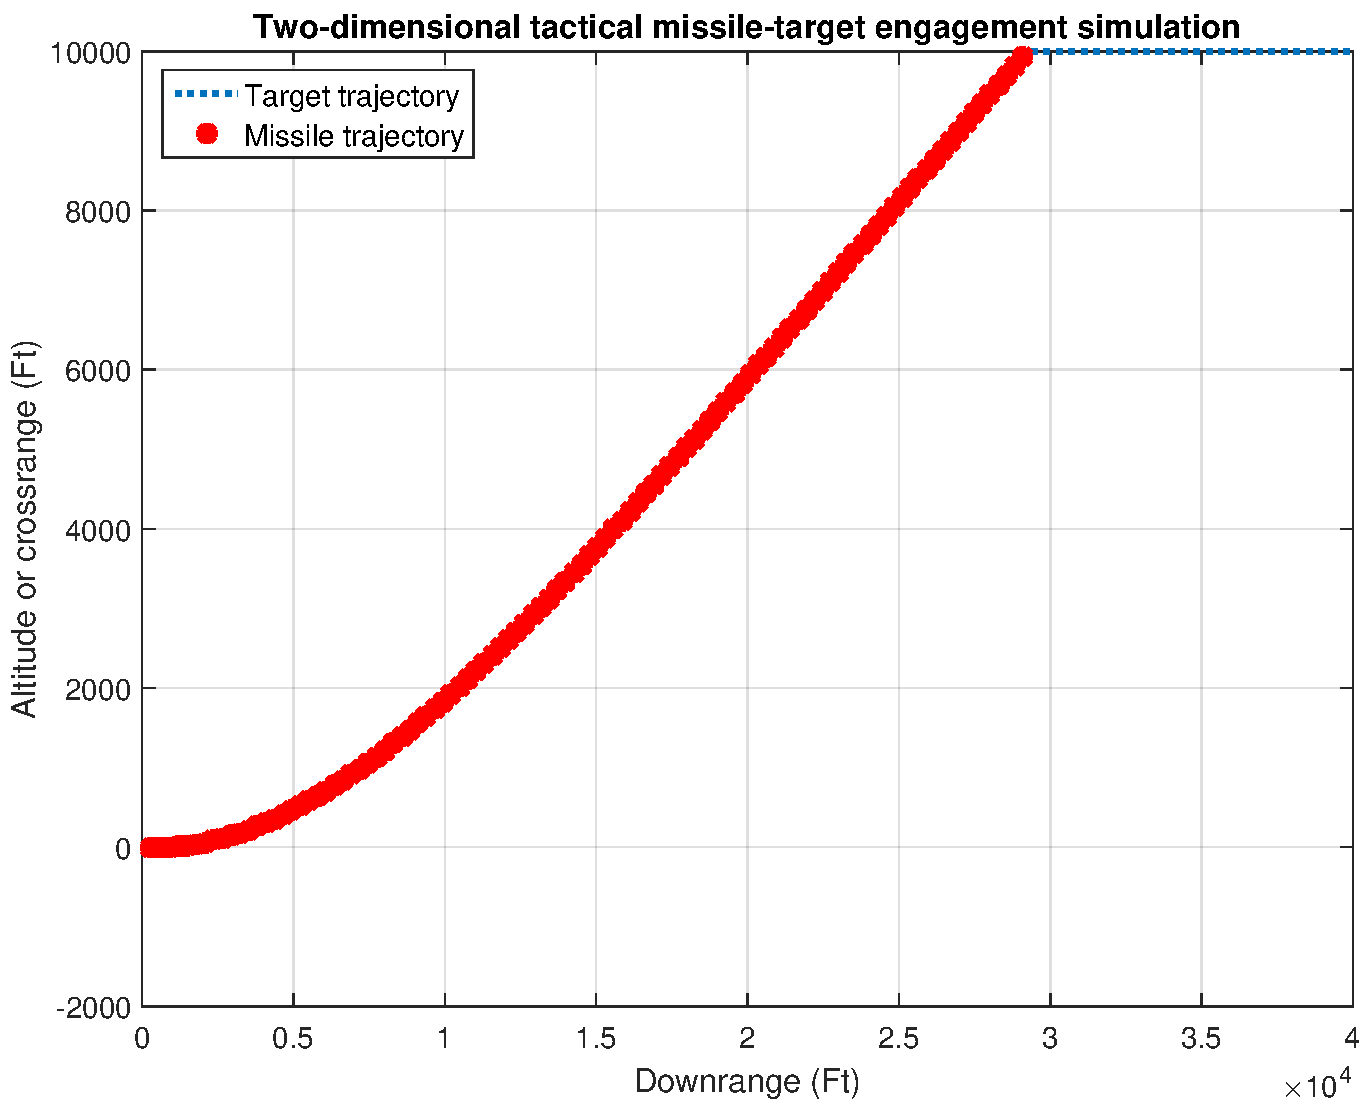
\includegraphics[scale = 0.57]{fig/trajectoryXNT0HE20N5.pdf}
	\caption{Trajectory of the target and attacker in case of zero target maneuver with heading error=-20 and $N'=5$.}
	\label{trajectory20N5}
\end{figure}


\begin{figure}[H]
	\centering
	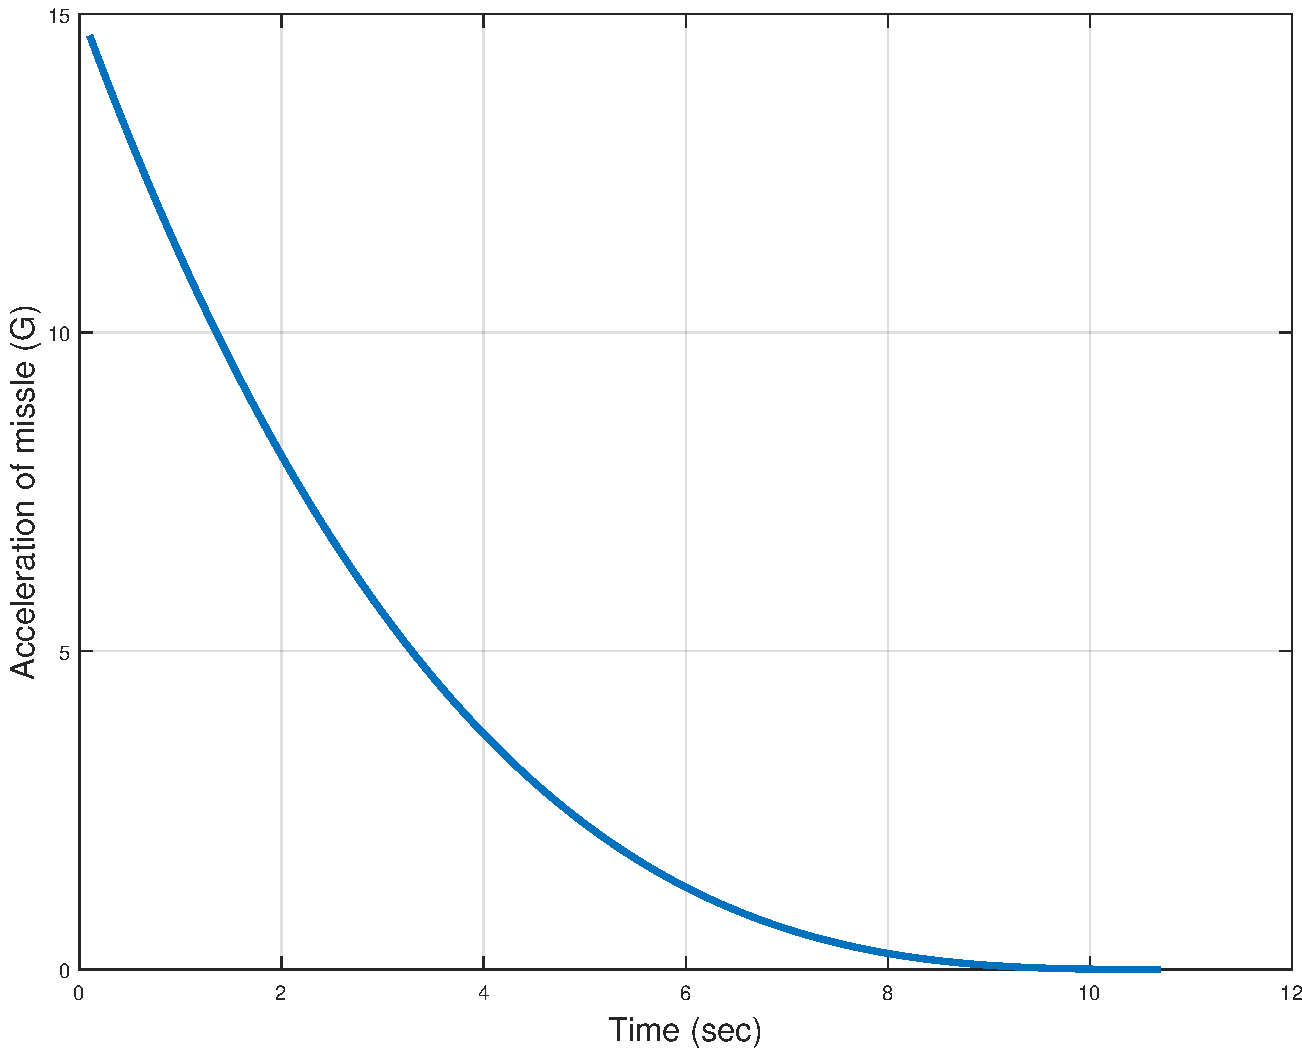
\includegraphics[scale = 0.57]{fig/MissileAccelerationXNT0HE20N5.pdf}
	\caption{Missile acceleration in case of zero target maneuver with heading error=-20 and $N'=5$ .}
	\label{missile acceleration20N5}
\end{figure}

%-----------------------------------------------------------

\subsubsection{Constant Target maneuver}
In this case the target does some effort to escape from the attacker, in the form of constant acceleration (in our example target acceleration = $5\ g$).
We see from Fig. \ref{missile acceleration0NN3} and Fig. \ref{missile acceleration0NN5} that a higher effective navigation ratio yields less acceleration to hit maneuvering target, and causes the missile to lead the target slightly more than a lower effective navigation ratio does, as we see from Fig. \ref{trajectory0NN3} and Fig. \ref{trajectory0NN5}.



\begin{figure}[htb]
	\centering
	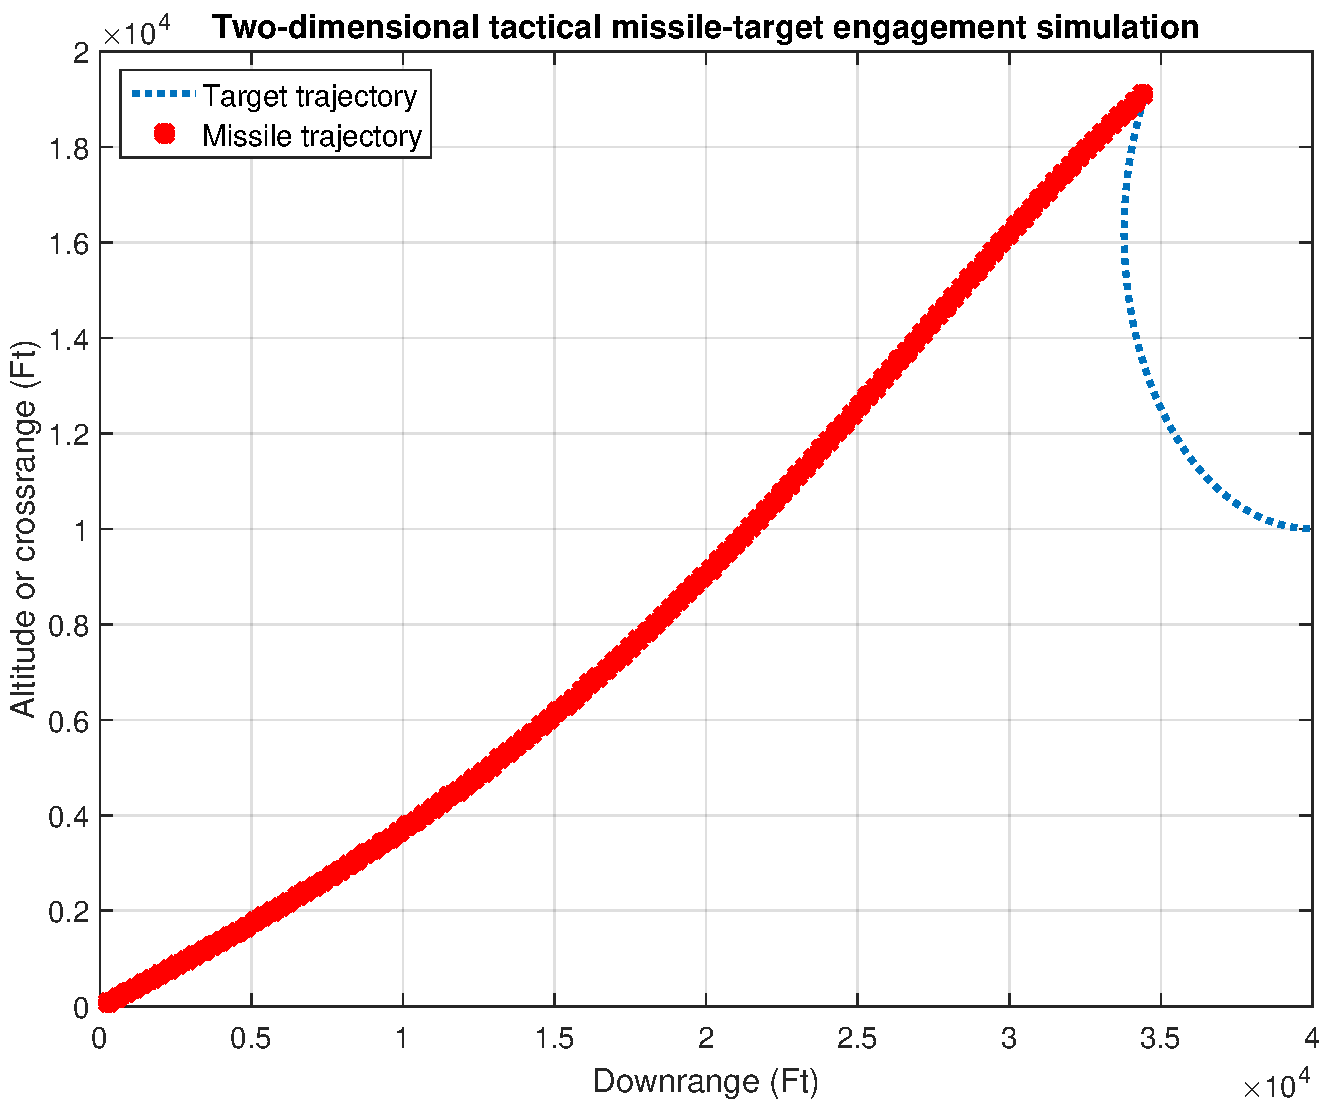
\includegraphics[scale = 0.75]{fig/trajectoryXNT5HE0N3.pdf}
	\caption{Trajectory of the target and attacker in case of constant target maneuver=5G with heading error=0 and $N'=3$.}
	\label{trajectory0NN3}
\end{figure}


\begin{figure}[htb]
	\centering
	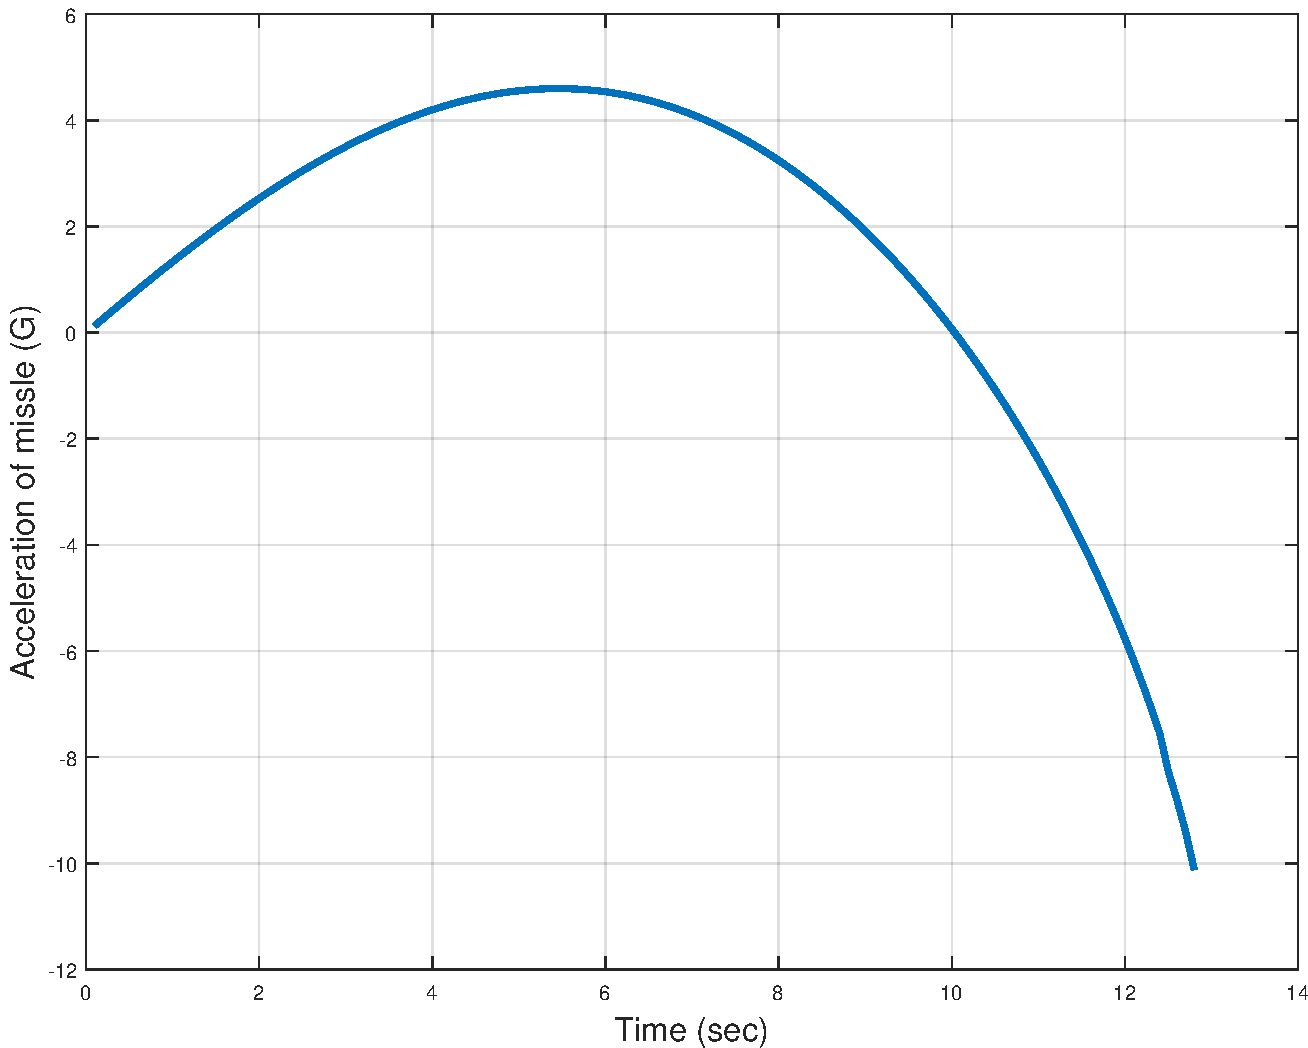
\includegraphics[scale = 0.65]{fig/MissileAccelerationXNT5HE0N3.pdf}
	\caption{Missile acceleration in case of constant target maneuver=5G with heading error=0 and $N'=3$ .}
	\label{missile acceleration0NN3}
\end{figure}

\begin{figure}[H]
	\centering
	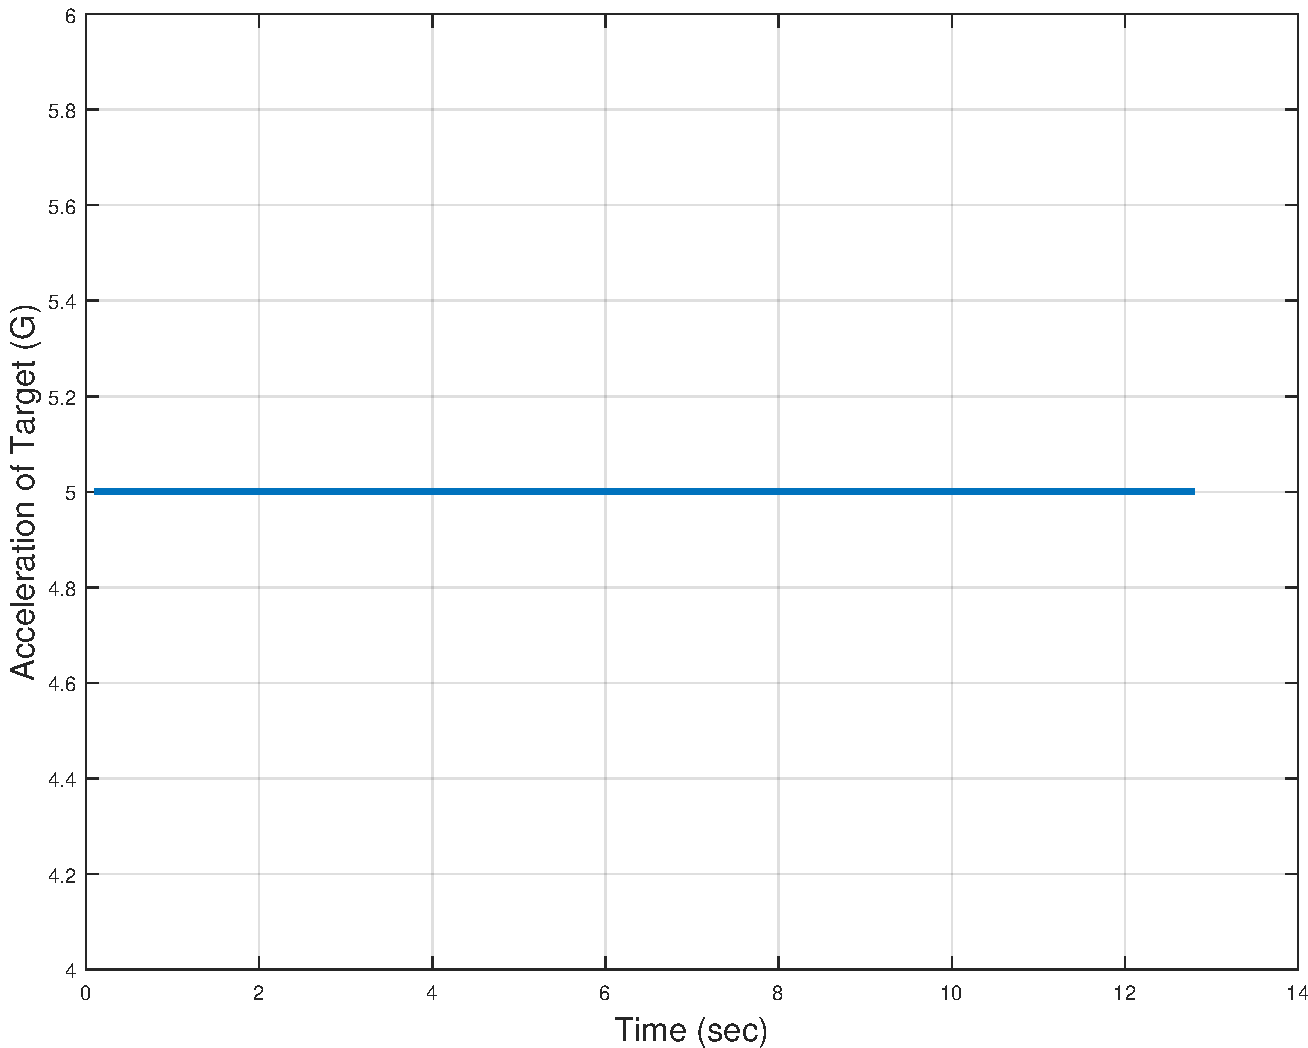
\includegraphics[scale = 0.65]{fig/TargetAccelerationXNT5HE0N3.pdf}
	\caption{Target acceleration in case of zero target maneuver with zero heading error and $N'=3$ .}
	\label{Target accelerationXNT5HE0N3}
\end{figure}


%----------

\begin{figure}[htb]
	\centering
	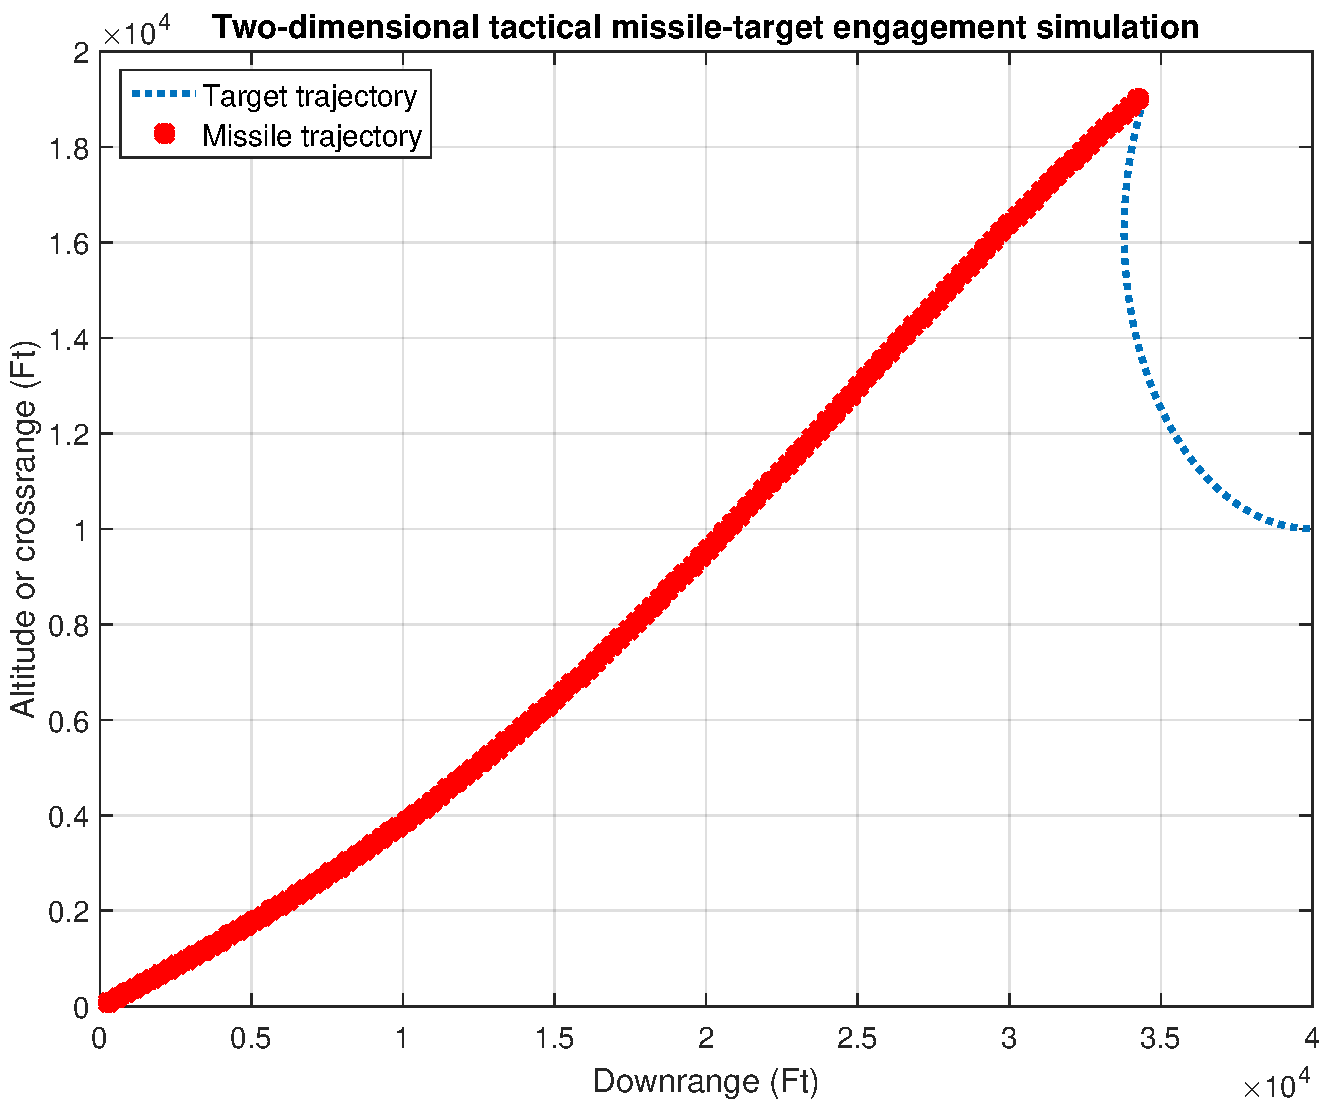
\includegraphics[scale = 0.35]{fig/trajectoryXNT5HE0N5.pdf}
	\caption{Trajectory of the target and attacker in case of constant target maneuver=5G with heading error=0 and $N'=5$.}
	\label{trajectory0NN5}
\end{figure}


\begin{figure}[htb]
	\centering
	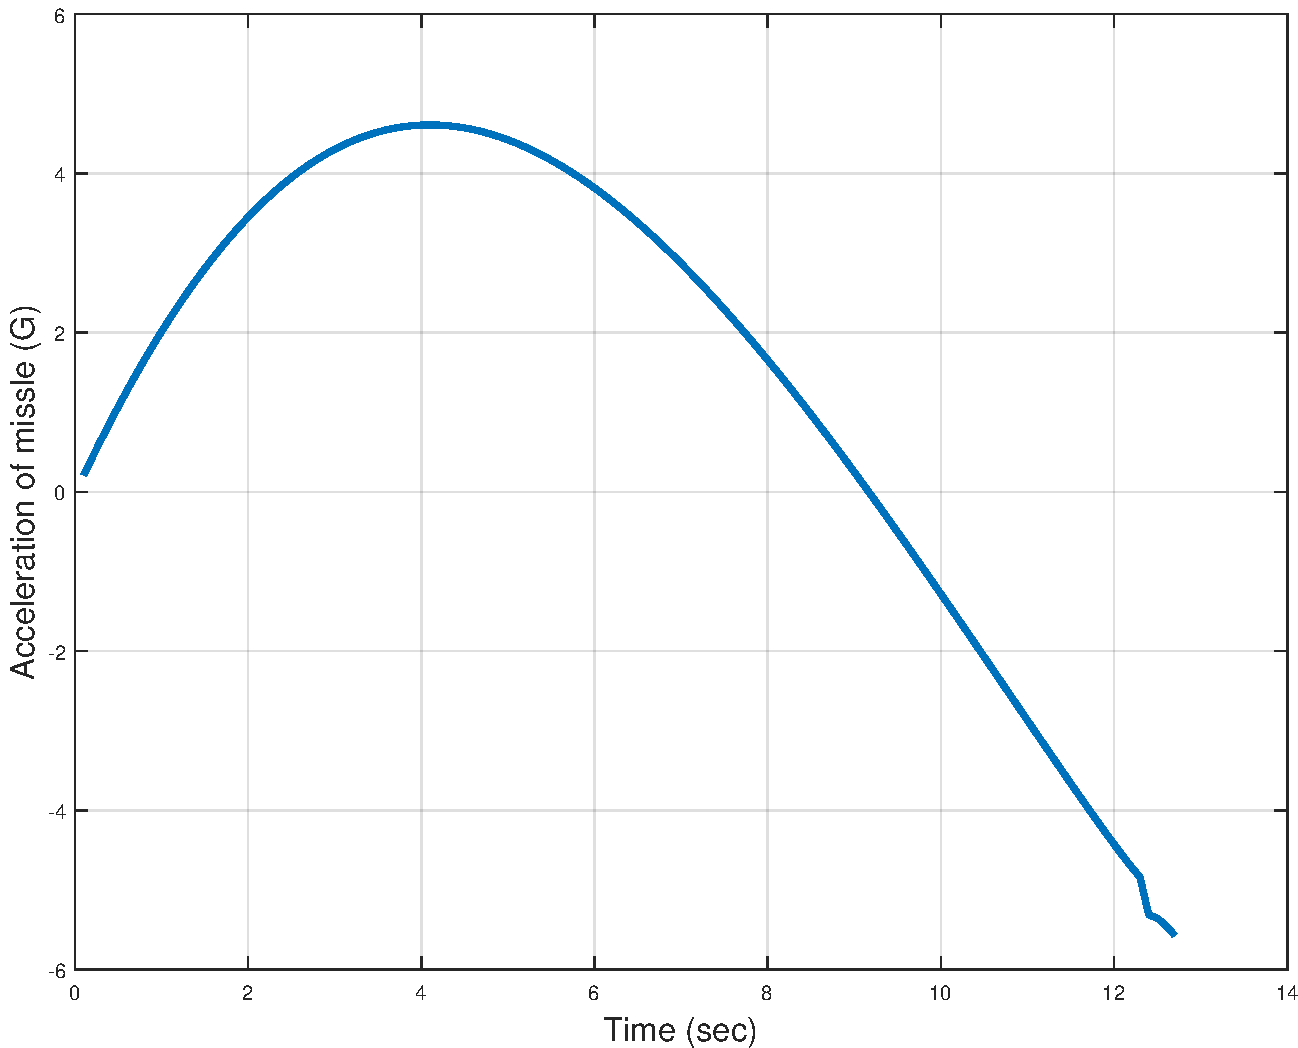
\includegraphics[scale = 0.35]{fig/MissileAccelerationXNT5HE0N5.pdf}
	\caption{Missile acceleration in case of constant target maneuver=5G with heading error=0 and $N'=5$ .}
	\label{missile acceleration0NN5}
\end{figure}


\begin{figure}[H]
	\centering
	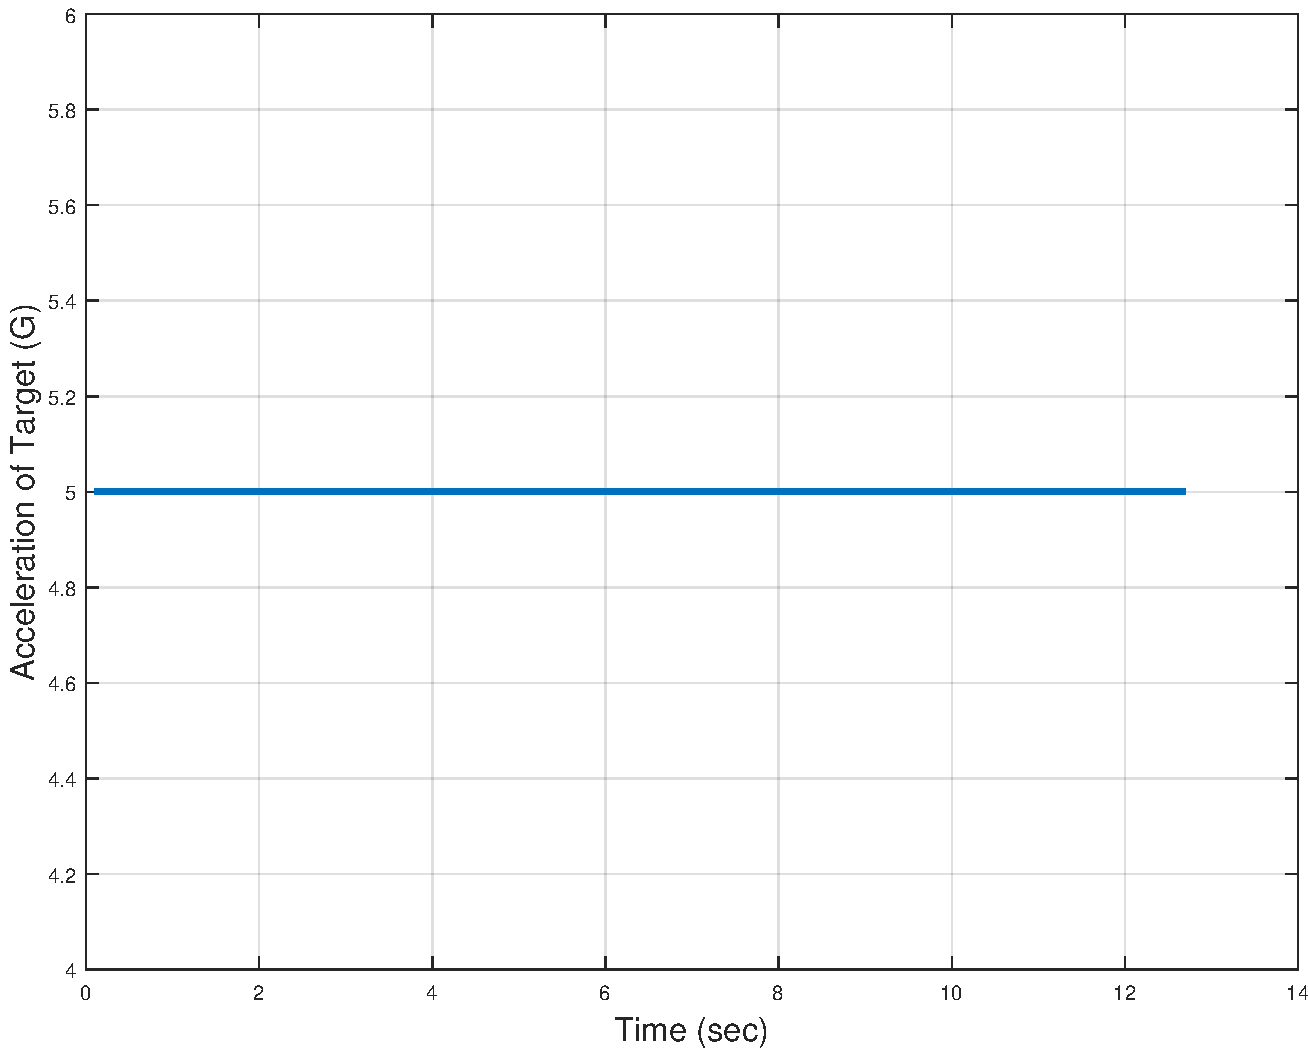
\includegraphics[scale = 0.35]{fig/TargetAccelerationXNT5HE0N5.pdf}
	\caption{Target acceleration in case of zero target maneuver with zero heading error and $N'=5$ .}
	\label{Target accelerationXNT5HE0N5}
\end{figure}

%-----------------------------------------------------------

\subsubsection{Polynomial Target maneuver}
Now we will make the Target maneuver as a polynomial in the form

\begin{equation}
f(t) = c_0 + c_1 T + c_2 T^2 + c_3 T^3 + ... + c_N T^N
\end{equation} 

where T is time, $ c_i$'s  are unknown coefficients of the polynomial and N is the polynomial degree.
In our simulation we choose N reasonably $3\to5$ and the coefficients are randomly generated then we solve the proportional navigation equations to get values for two important parameters, namely the miss distance and the command acceleration for the Missile. Then, we calculate the cost function depends on these two parameters, as our target is to maximize miss distance to make the target safe, and maximize command acceleration for the missile, so it bleeds energy before it catches the target. We will do this process many times till the number of runs we need. The next figures shows the trajectories of the Target and Missile for N=3,4 and corresponding missile and target accelerations for each case.
In the first case (N=3), as we see from Fig. \ref{Target accelerationP3N3} the target have to exert $50 G$ to escape from the attacker, these amount of G'es is very high and the pilot could not withstand all this amount. Also, form Fig. \ref{missile accelerationP3} the attacker have to exert 120 G, this will not happen and the missile's energy will bleed at 100 G after 5 sec. Here the simulation did not till us a complete vision about what will happen. We have to take in consideration the amount of G's that the pilot could resist, so we will use genetic algorithm technique to generate the polynomial because it is easy to control the maximum target acceleration in this method.
The second case (N=4), is hypothetical case because the pilot will die in less than 1 sec. If the technology improved and the scientists invent a pilot suit that could resist these huge amount of G'es, then we can take this solution in consideration.        

\begin{figure}[H]
	\centering
	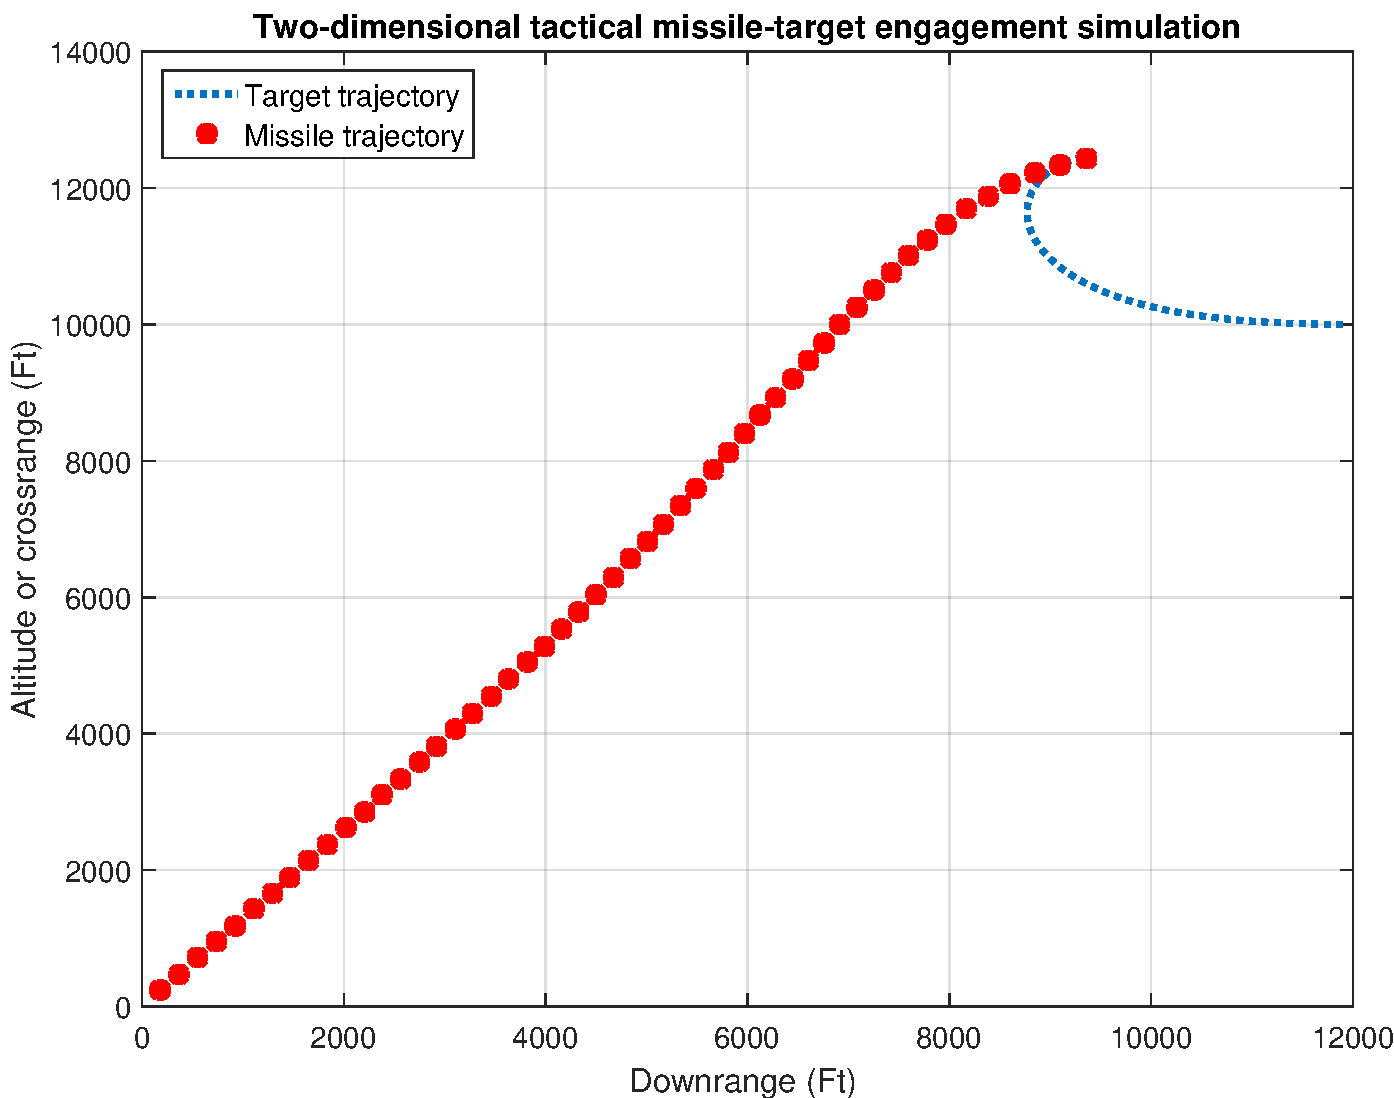
\includegraphics[scale = 0.55]{fig/trajectoryP3N3.pdf}
	\caption{Trajectory of the target and attacker in case of polynomial of degree N=3 target maneuver with zero heading error and $N'=3$.}
	\label{trajectoryP3}
\end{figure}


\begin{figure}[H]
	\centering
	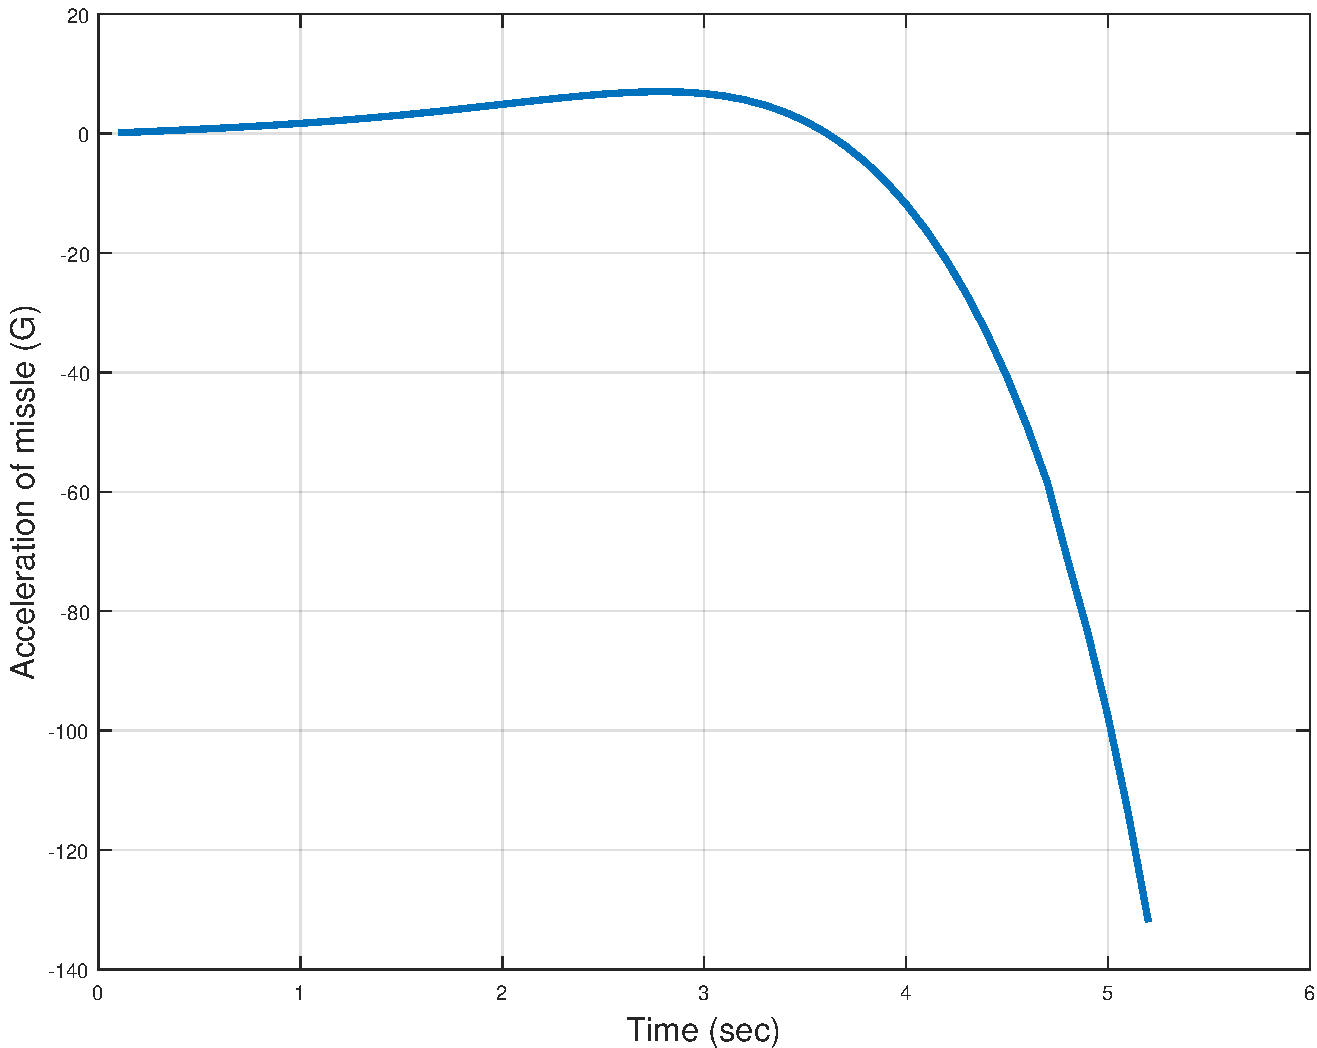
\includegraphics[scale = 0.55]{fig/MissileAccelerationP3N3.pdf}
	\caption{Missile acceleration in case of  polynomial of degree N=3 target maneuver with zero heading error and $N'=3$.}
	\label{missile accelerationP3}
\end{figure}


\begin{figure}[H]
	\centering
	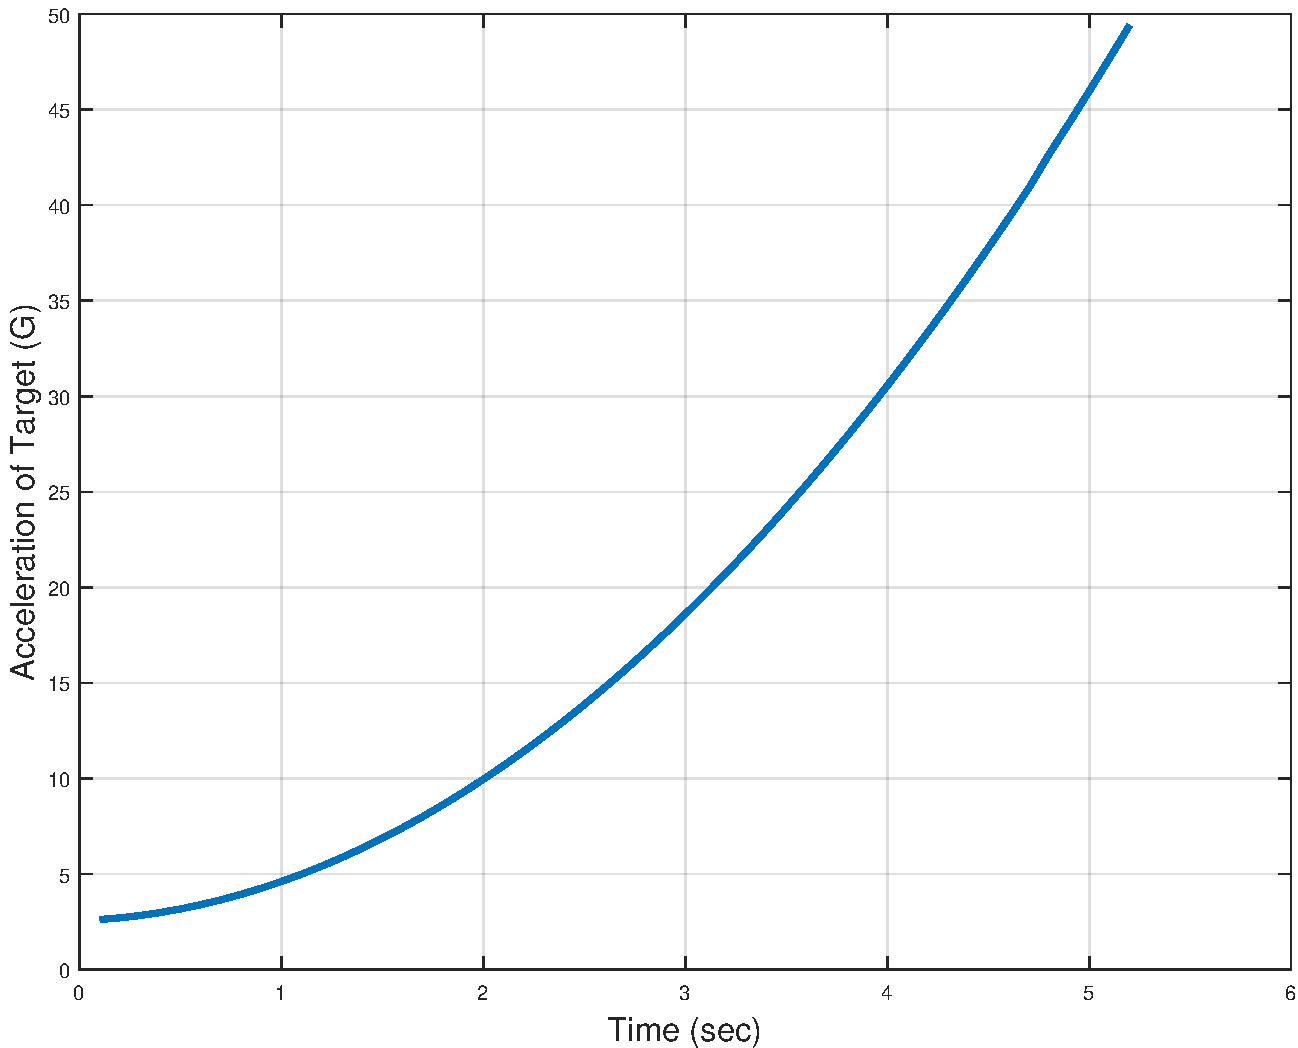
\includegraphics[scale = 0.55]{fig/TargetAccelerationP3N3.pdf}
	\caption{Target acceleration in case of  polynomial of degree N=3 target maneuver with zero heading error and $N'=3$.}
	\label{Target accelerationP3N3}
\end{figure}

%----------
\begin{figure}[htb]
	\centering
	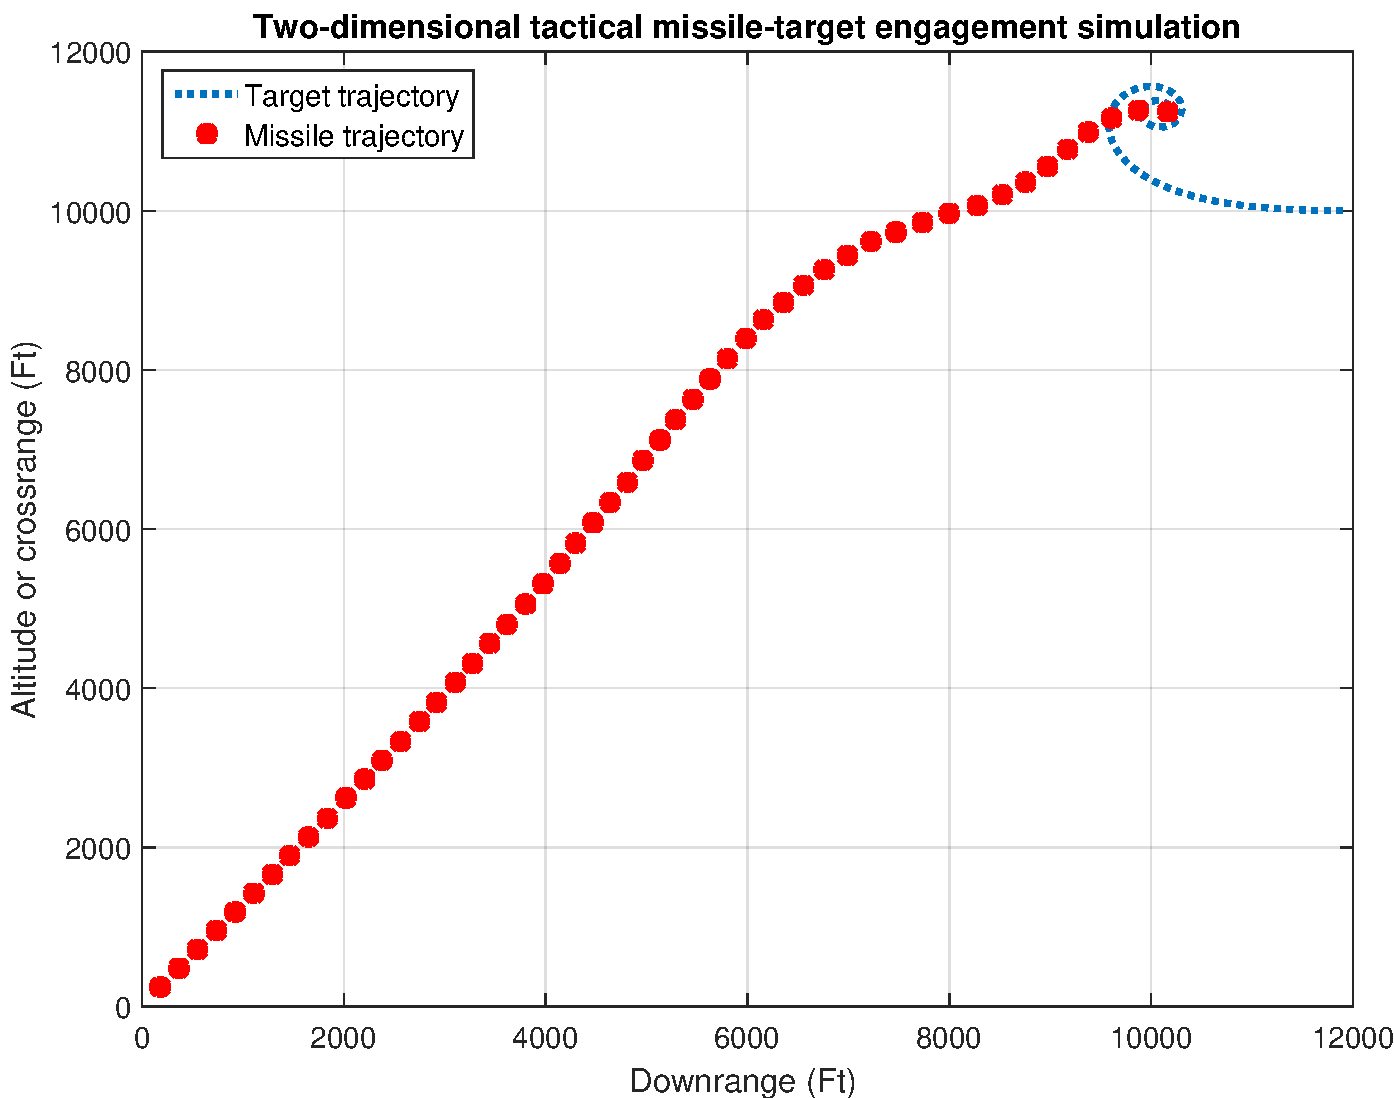
\includegraphics[scale = 0.35]{fig/trajectoryP4N3.pdf}
	\caption{Trajectory of the target and attacker in case of  polynomial of degree N=4 target maneuver with zero heading error and $N'=3$.}
	\label{trajectoryP4}
\end{figure}


\begin{figure}[htb]
	\centering
	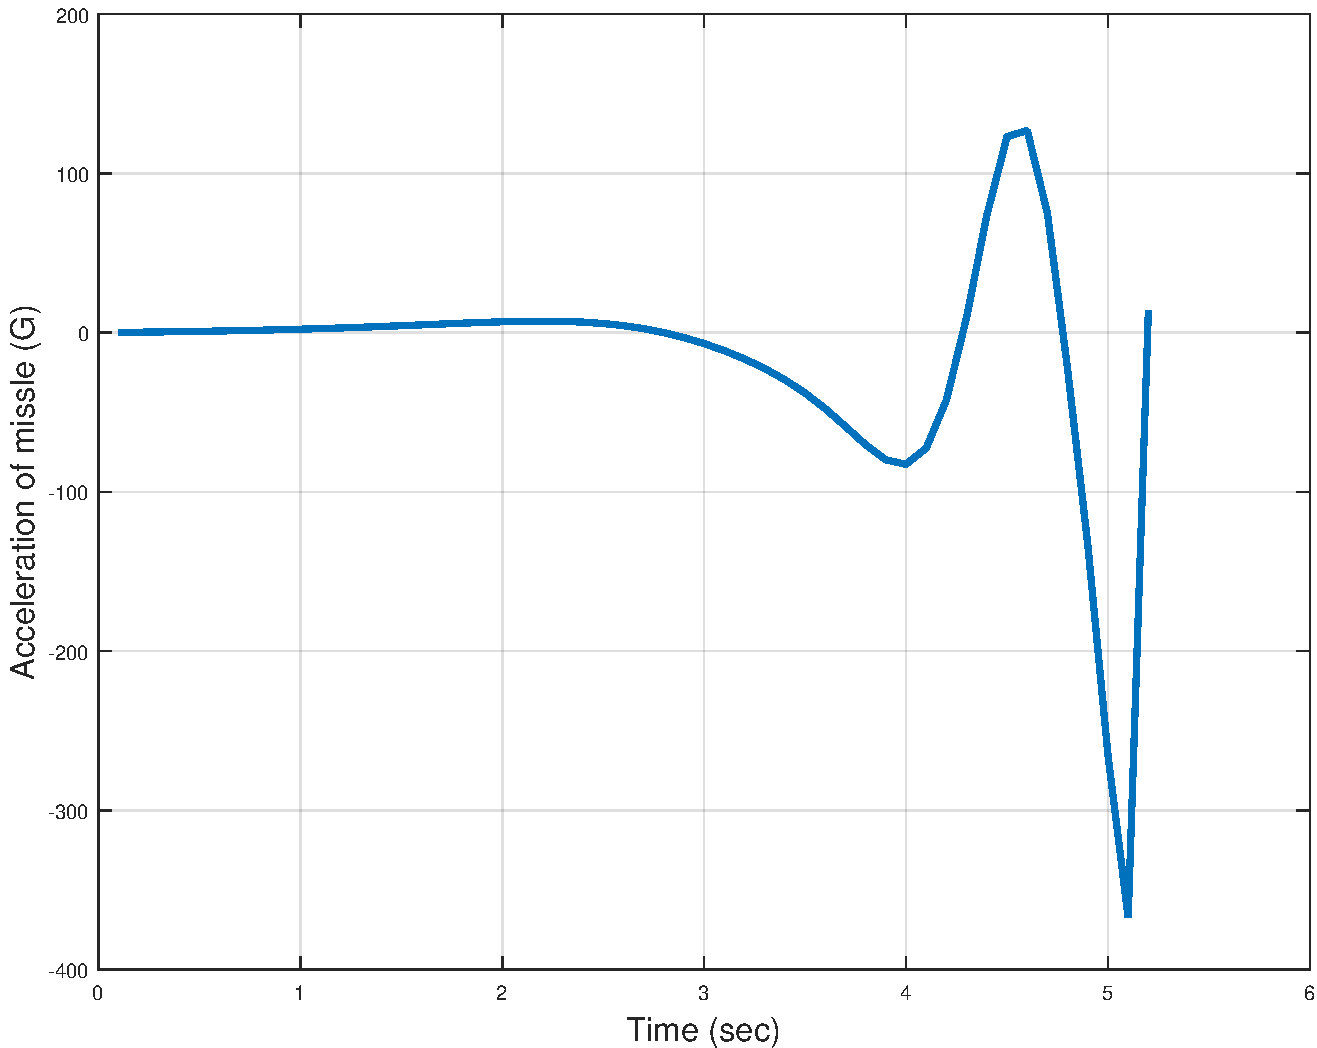
\includegraphics[scale = 0.35]{fig/MissileAccelerationP4N3.pdf}
	\caption{Missile acceleration in case of  polynomial of degree N=4 target maneuver with zero heading error and $N'=3$.}
	\label{missile accelerationP4}
\end{figure}

\begin{figure}[H]
	\centering
	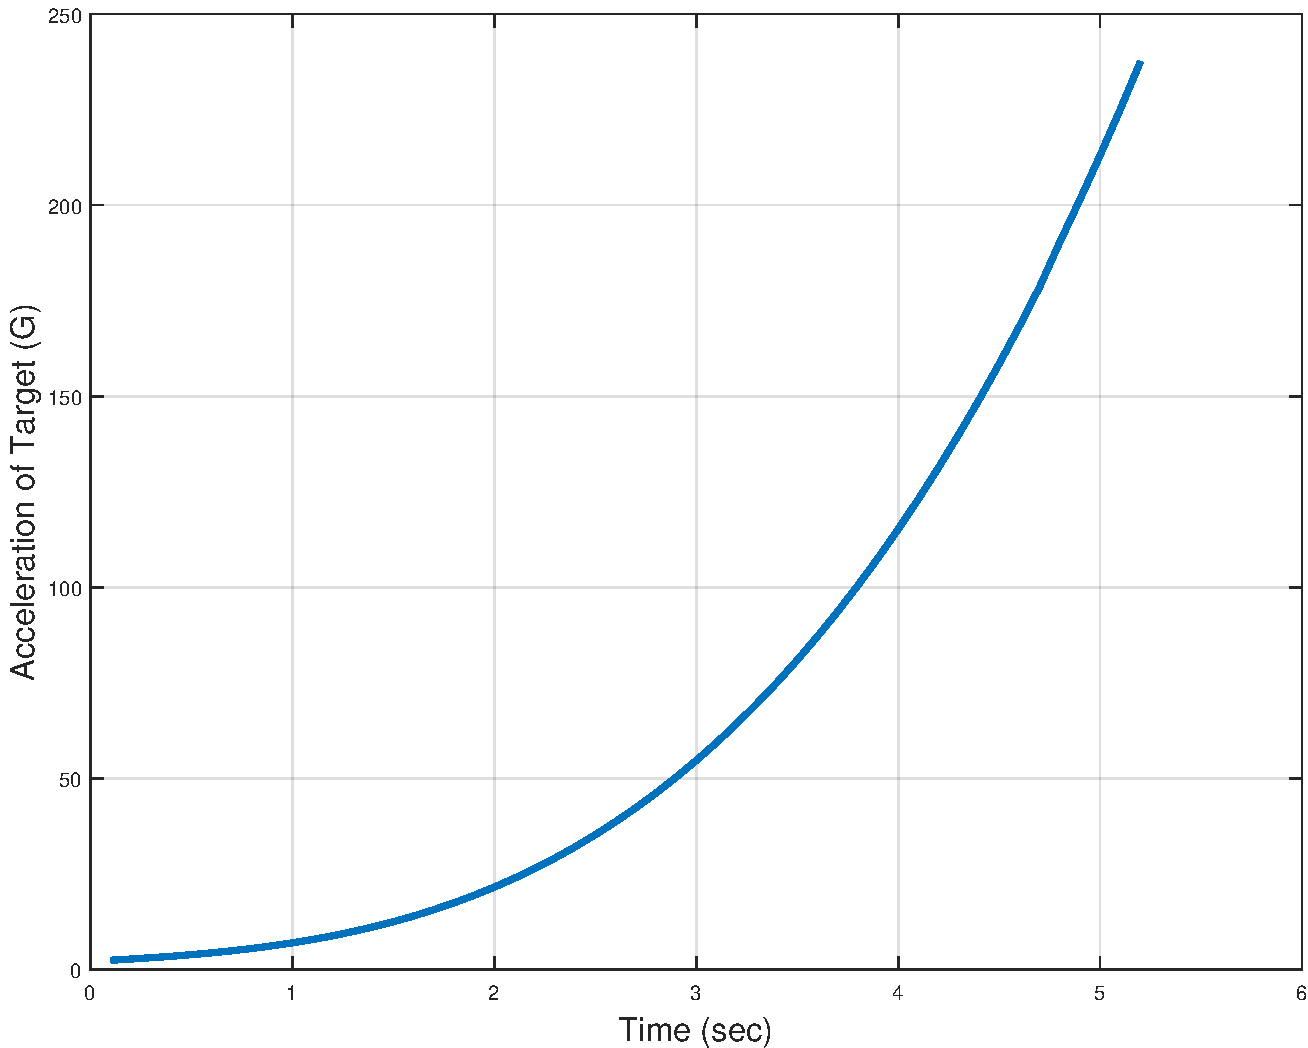
\includegraphics[scale = 0.35]{fig/TargetAccelerationP4N3.pdf}
	\caption{Target acceleration in case of  polynomial of degree N=4 target maneuver with zero heading error and $N'=3$.}
	\label{Target accelerationP4N3}
\end{figure}


%------------------------------------------------------------

\subsubsection{Trapezoidal Target maneuver}
Now we will make the Target maneuver as a trapezoidal function (as a general case of tooth and square maneuvers) illustrated in Fig. \ref{trapezoidalacc}


\begin{figure}[htb]
	\centering
	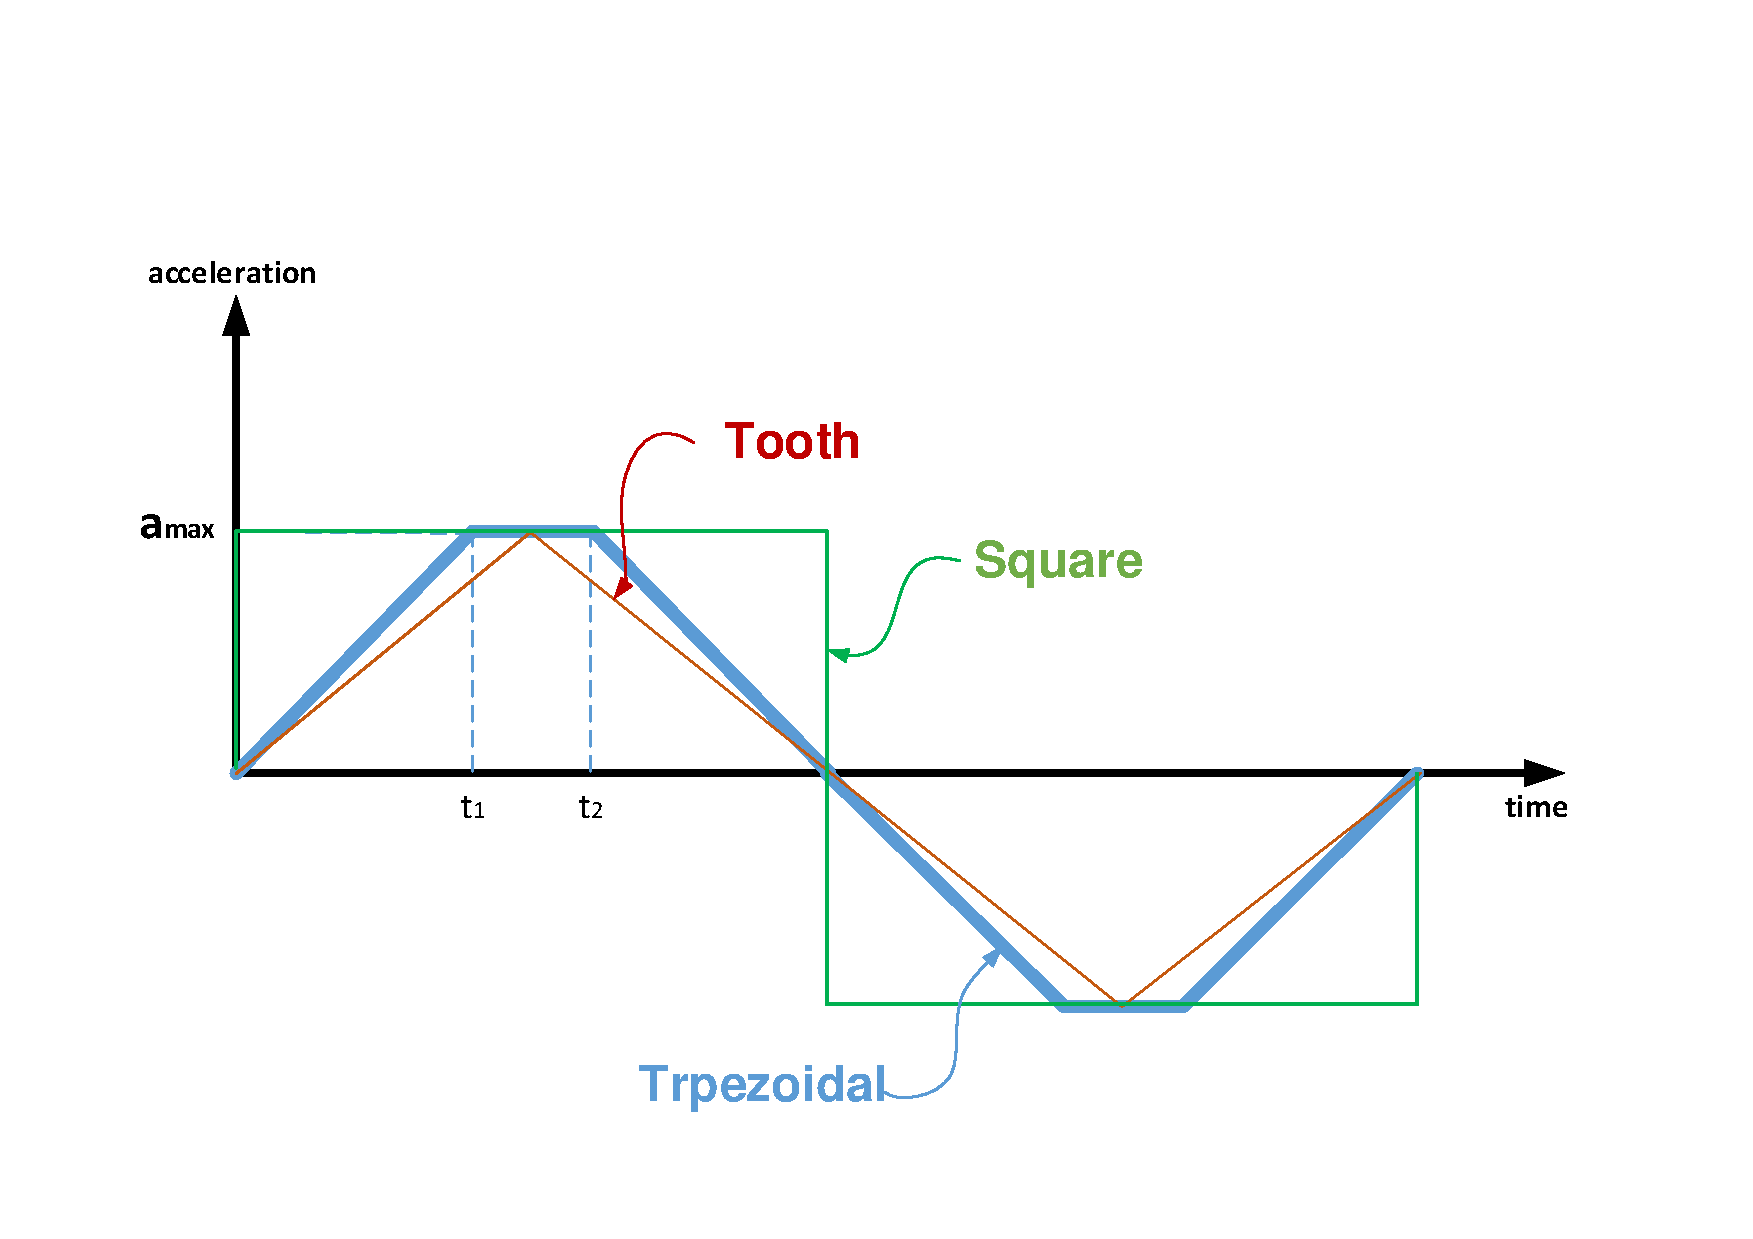
\includegraphics[scale = 0.60]{fig/toothSquareTrapezoidal.pdf}
	\caption{Trapezoidal Target maneuver.}
	\label{trapezoidalacc}
\end{figure}
In the simulation we choose the value for maximum acceleration. The time of beginning the ramp (which is 0), and the time at the end of the descent, $t_1$ and $t_2$ are variables. 

We have two cases: \textbf{First case:} the maneuver is \textit{symmetric} so we have two extreme cases.
\begin{itemize}
	\item when $t_1$ is equal to zero (there is no ascend ramp)  so $t_2$ is at the middle of the maneuver; this leads to \textit{square} target maneuver.
	\item when $t_1$ equals $t_2$ at the quarter of the maneuver; this leads to \textit{tooth} target maneuver.  
\end{itemize}
Varying $t_1$ and $t_2$, starting from the square case till the tooth case, until we find the optimum solution based on or cost function which depends on the values of the miss distance and Missile acceleration. 

%------------
\begin{figure}[htb]
	\centering
	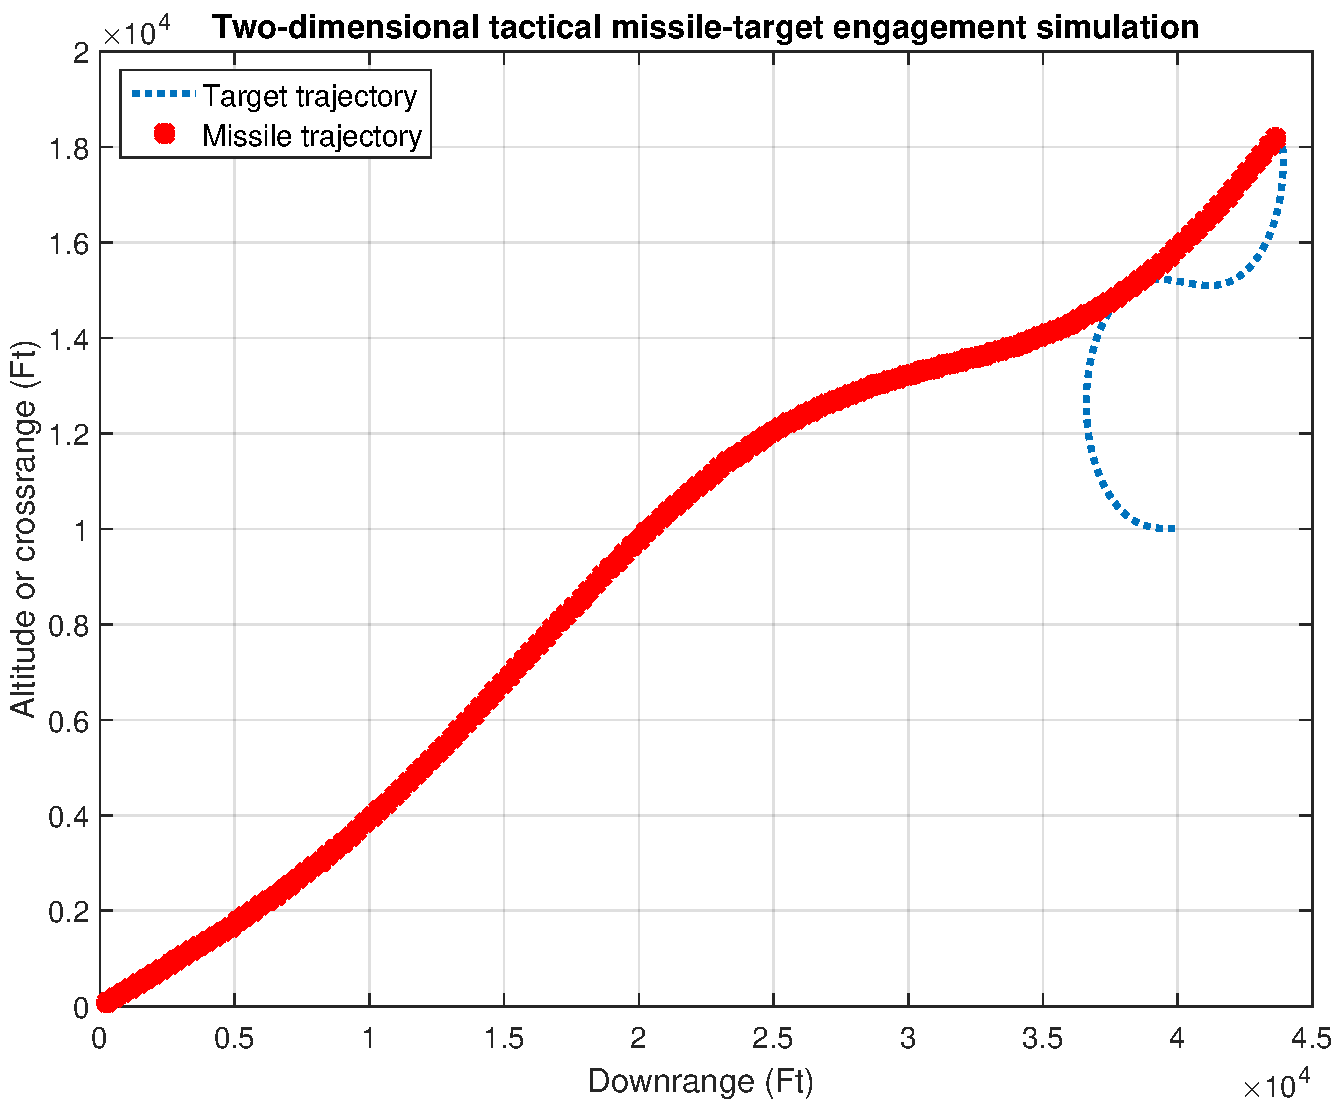
\includegraphics[scale = 0.35]{fig/trajectoryTrapSymm.pdf}
	\caption{Trajectory of the target and attacker in case of symmetric trapezoidal target maneuver with zero heading error and $N'=5$.}
	\label{trajectory trapSymm}
\end{figure}


\begin{figure}[htb]
	\centering
	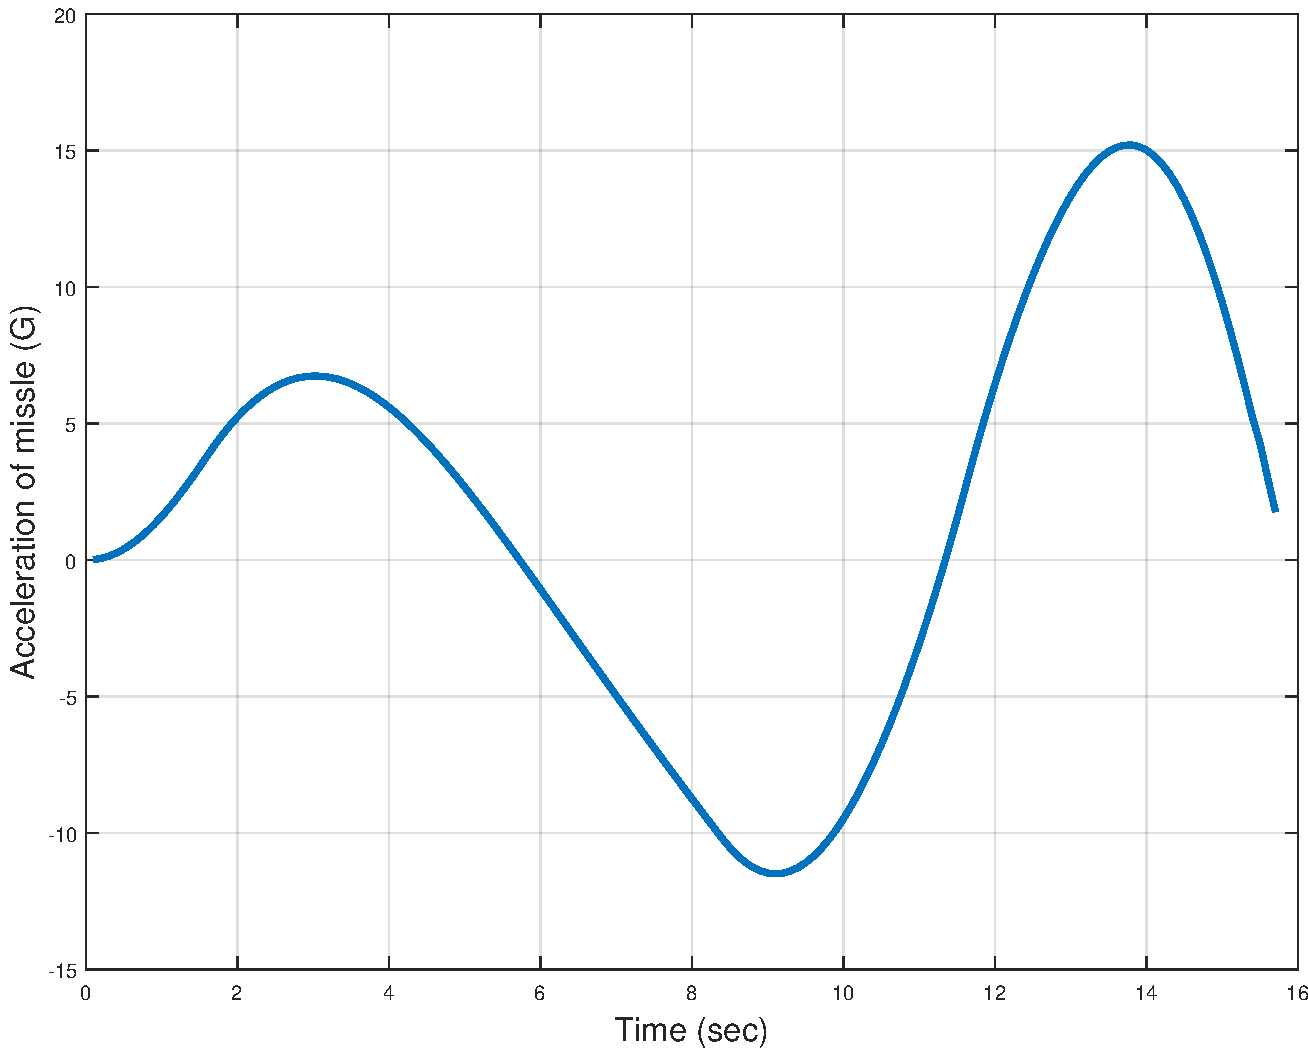
\includegraphics[scale = 0.35]{fig/MissileAccelerationTrapSymm.pdf}
	\caption{Missile acceleration in case of symmetric trapezoidal target maneuver with zero heading error and $N'=5$.}
	\label{missile acceleration trapSymm}
\end{figure}

\begin{figure}[H]
	\centering
	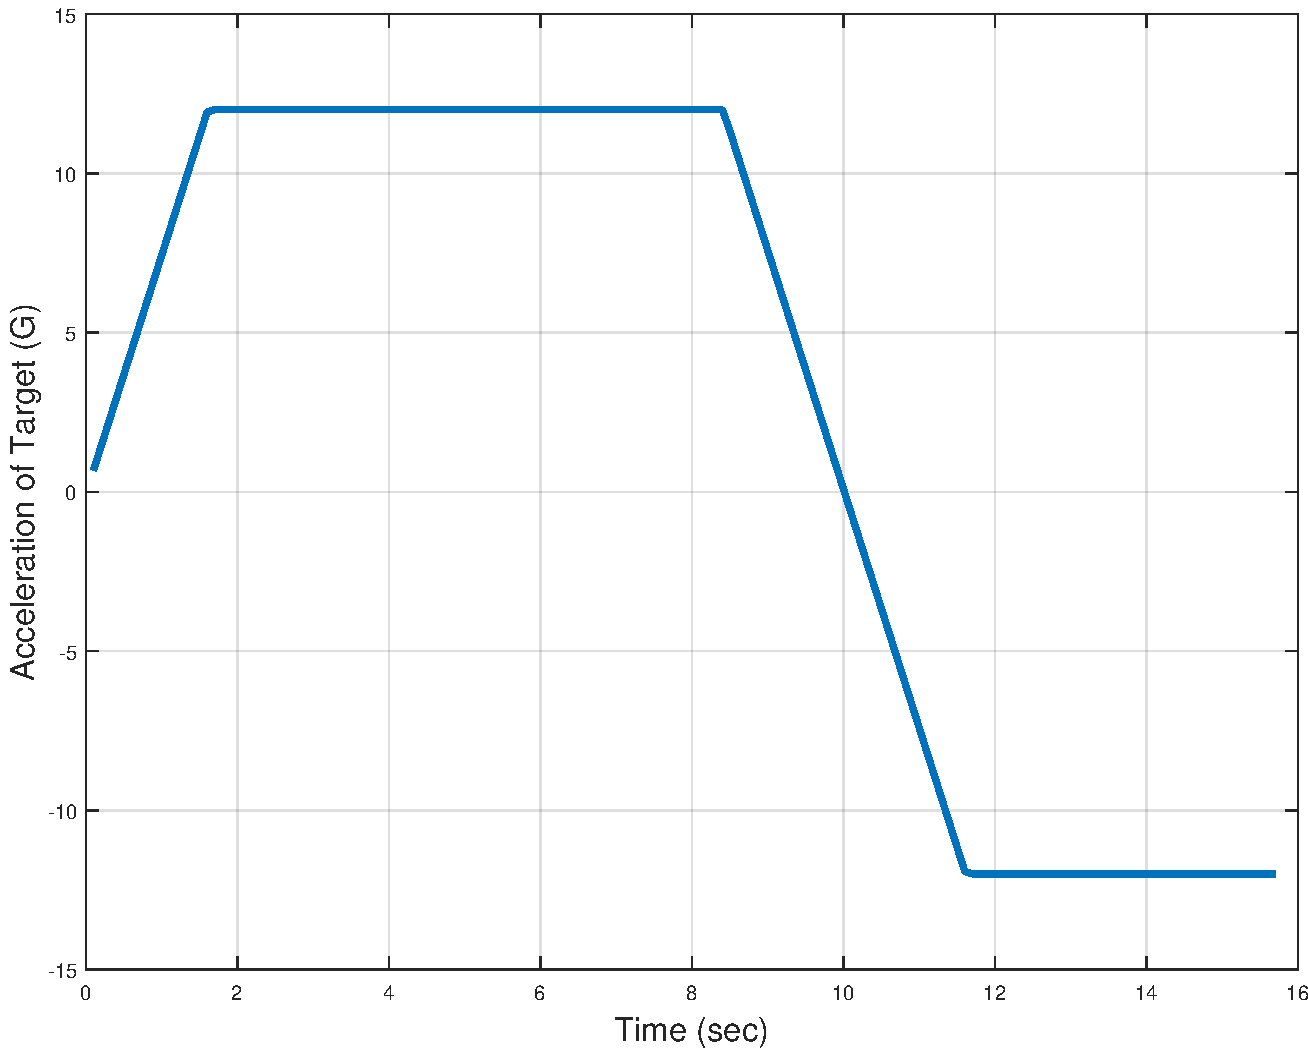
\includegraphics[scale = 0.35]{fig/TargetAccelerationTrapSym.pdf}
	\caption{Target acceleration in case of symmetric trapezoidal N=4 target maneuver with zero heading error and $N'=5$.}
	\label{Target acceleration trapSymm}
\end{figure}

%----------

\textbf{Second case:} the maneuver is \textit{not symmetric} so we put a first value for $t_1$ (starting with zero) and varying $t_2$ till we scan all the domain, then change $t_1$ slightly and scan all the domain again with $t_2$ till we find the optimum solution.

What about if the optimum solution for the target maneuver did not have Identical halves? and all the slops are not related to each other. We will try to figure that using genetic algorithm in the next section. 


%------------
\begin{figure}[htb]
	\centering
	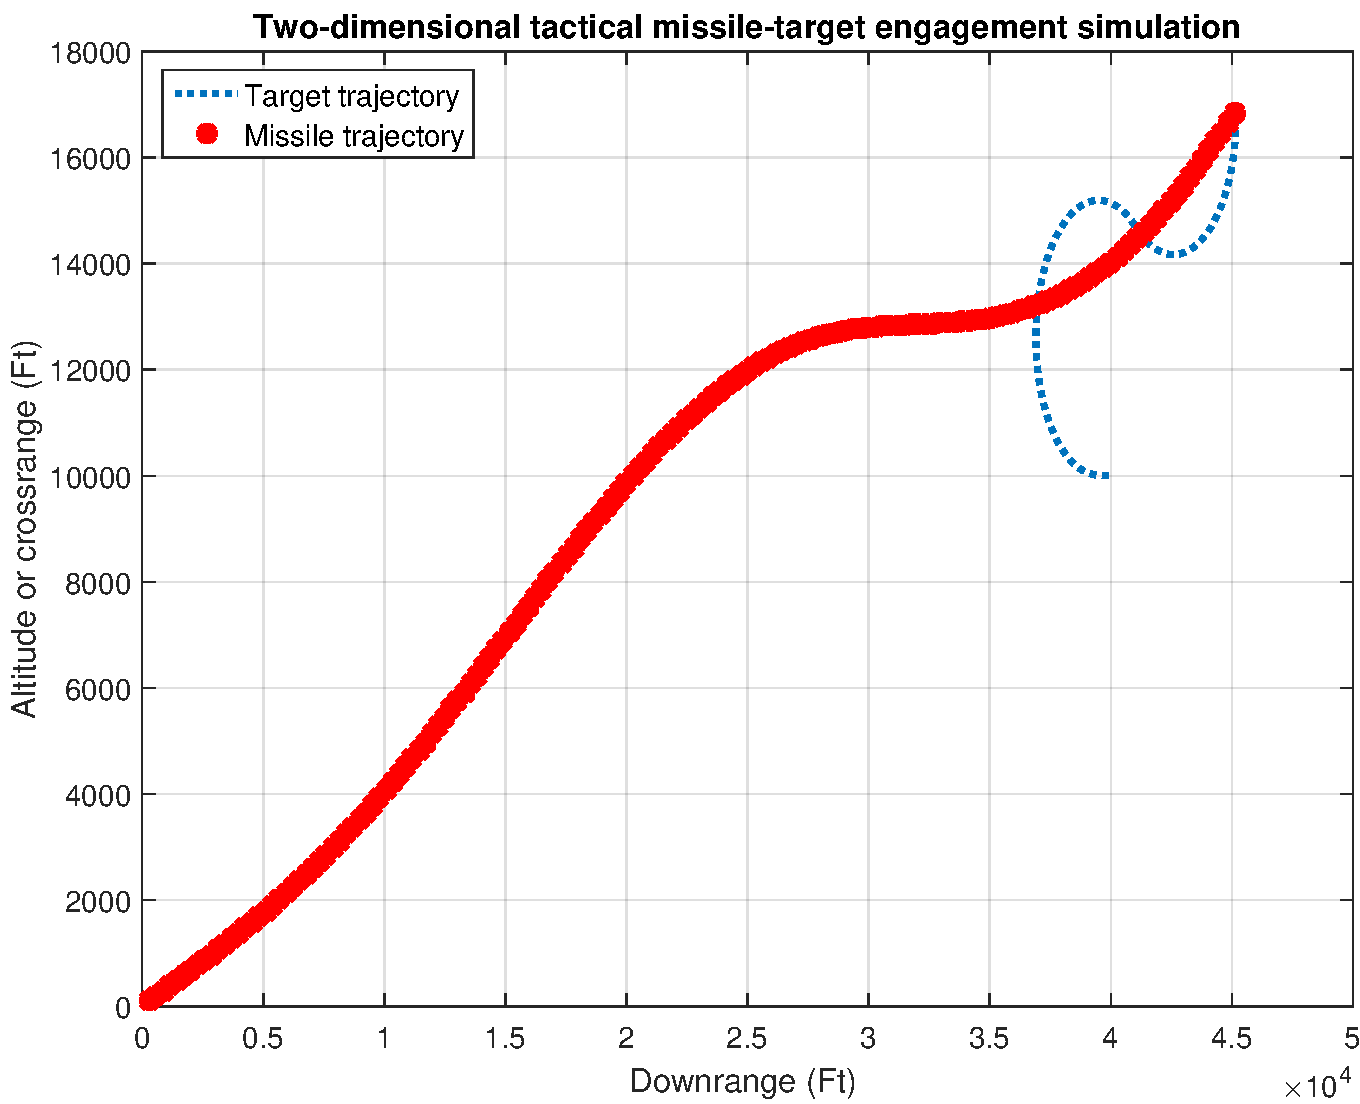
\includegraphics[scale = 0.35]{fig/trajectoryTrap.pdf}
	\caption{Trajectory of the target and attacker in case of trapezoidal target maneuver with zero heading error and $N'=5$.}
	\label{trajectory trap}
\end{figure}


\begin{figure}[htb]
	\centering
	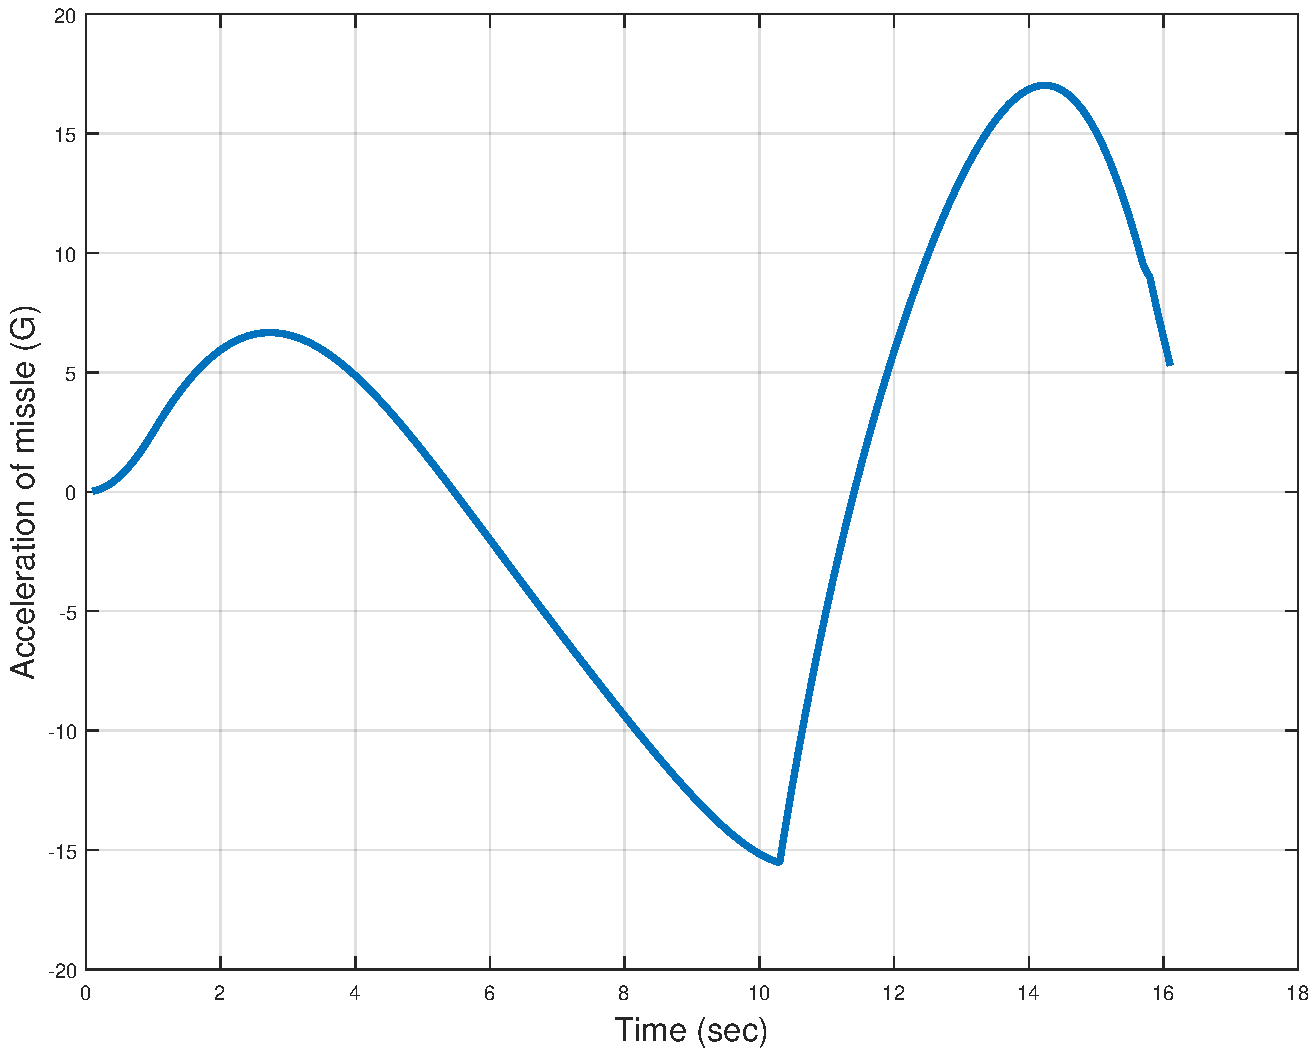
\includegraphics[scale = 0.35]{fig/MissileAccelerationTrap.pdf}
	\caption{Missile acceleration in case of trapezoidal target maneuver with zero heading error and $N'=5$.}
	\label{missile acceleration trap}
\end{figure}

\begin{figure}[H]
	\centering
	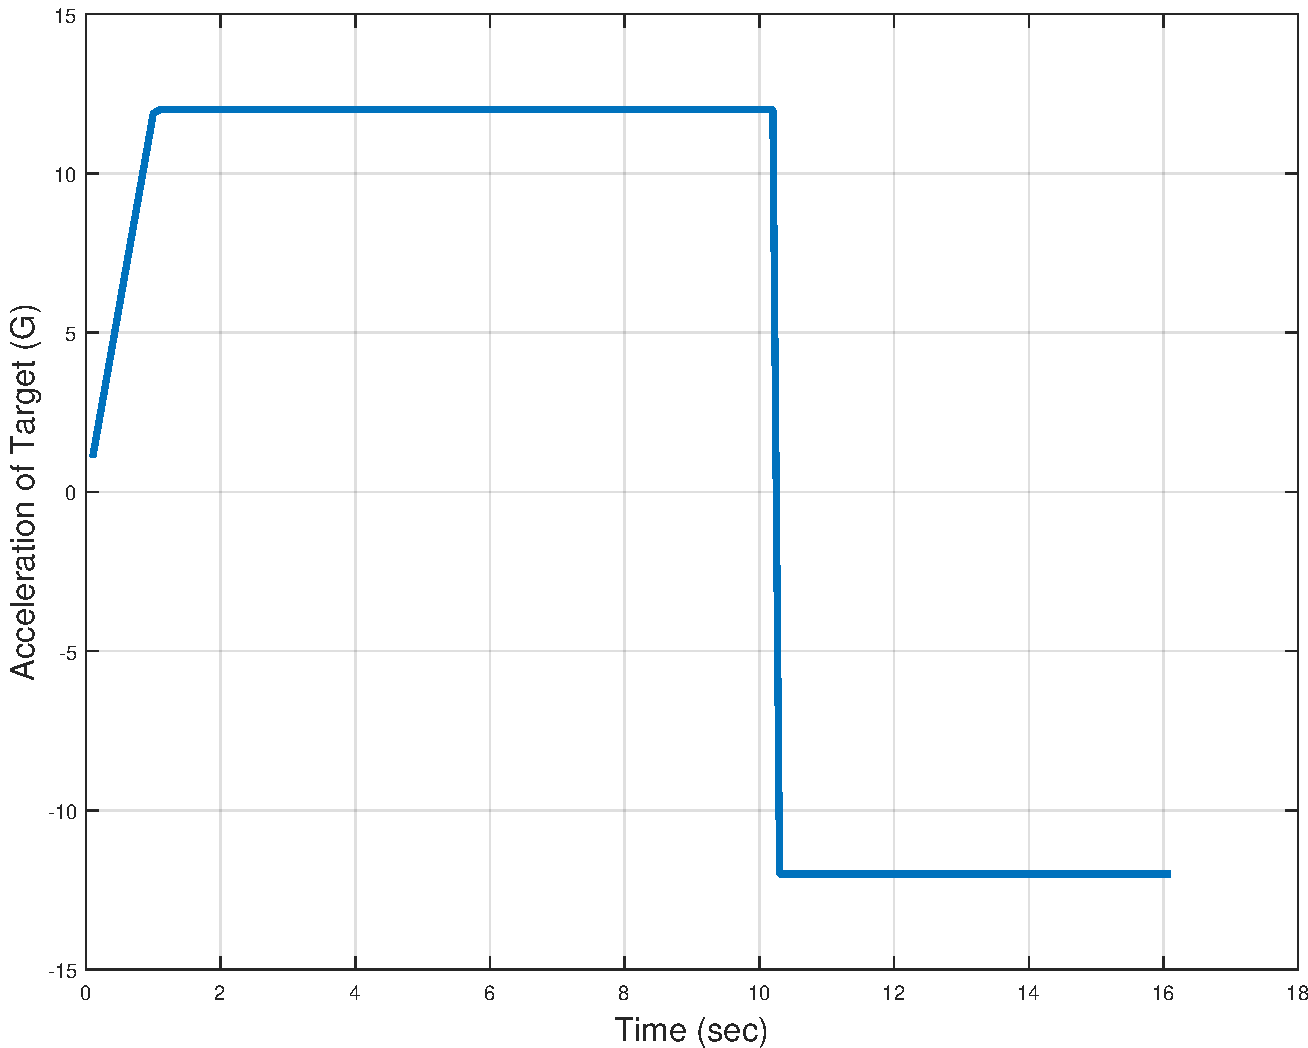
\includegraphics[scale = 0.35]{fig/TargetAccelerationTrap.pdf}
	\caption{Target acceleration in case of trapezoidal N=4 target maneuver with zero heading error and $N'=5$.}
	\label{Target acceleration trap}
\end{figure}

%----------
%=================================================================================

\section{Guidance Toolbox}

All the previous results could be generated from a simple GUI (graphic user interface), (Fig.\ref{Guidance Toolbox}).  The inputs for this GUI are the locations and velocities for the Target (plane) and the Attacker (missile). Then the user have to choose the guidance law (this will be as a future work, till now we have only PN guidance law), which is the way that the Attacker tracking the Target.

\begin{figure}[H]
	\centering
	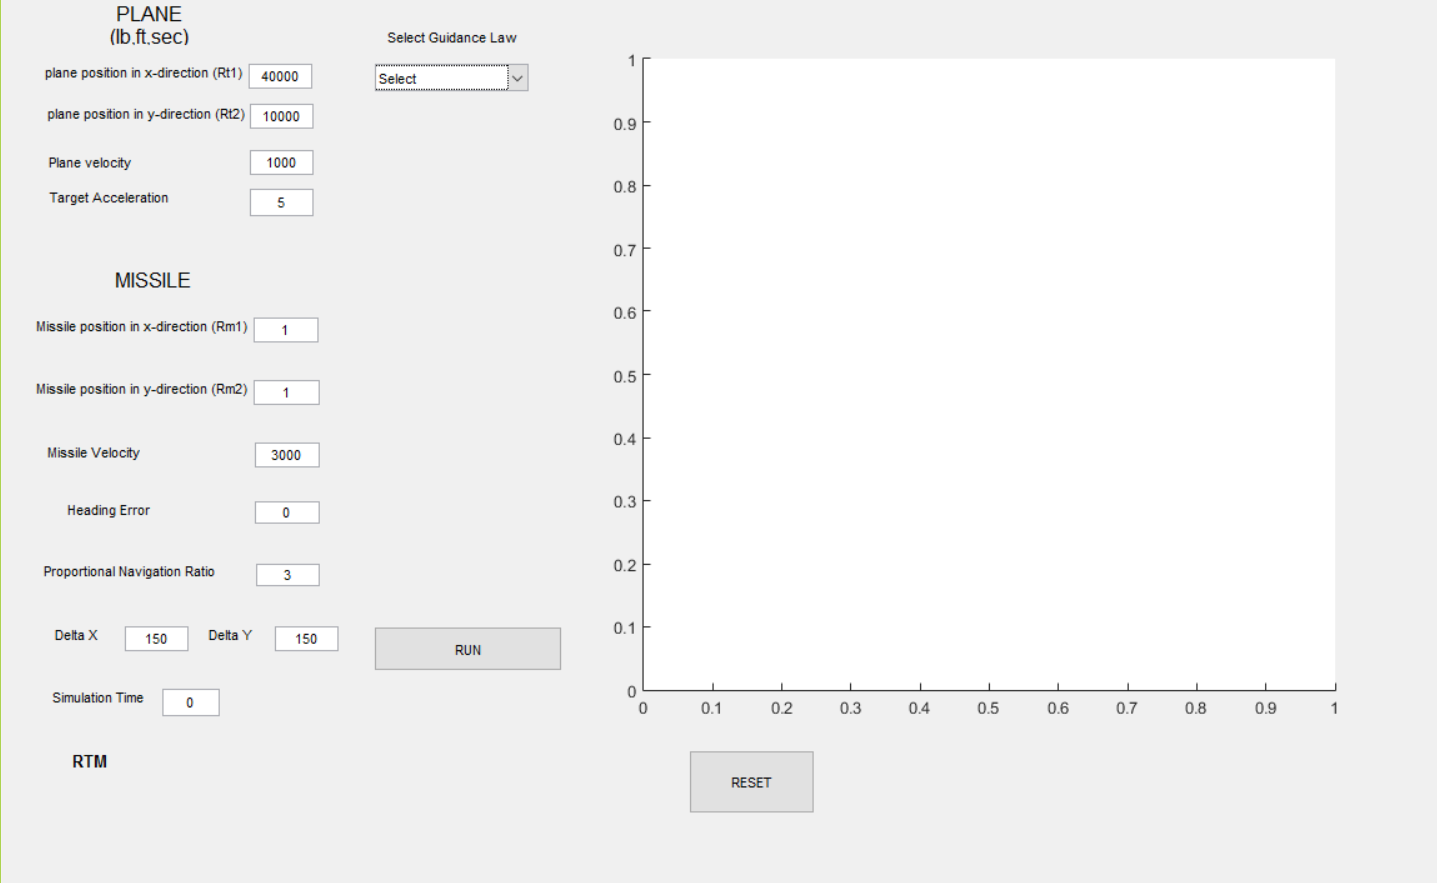
\includegraphics[scale = 0.45]{fig/GUI.PNG}
	\caption{Guidance Toolbox}
	\label{Guidance Toolbox}
\end{figure}


If the user chooses the PN guidance law (Fig.\ref{Guidance Toolbox PN}) , there will be more options be available, Now he could select the type of escape maneuver:
\begin{itemize}
	\item Polynomial
	\item Trapezoidal
	\item Symmetric Trapezoidal
\end{itemize}

and the result will be optimized escape maneuver. 

\begin{figure}[H]
	\centering
	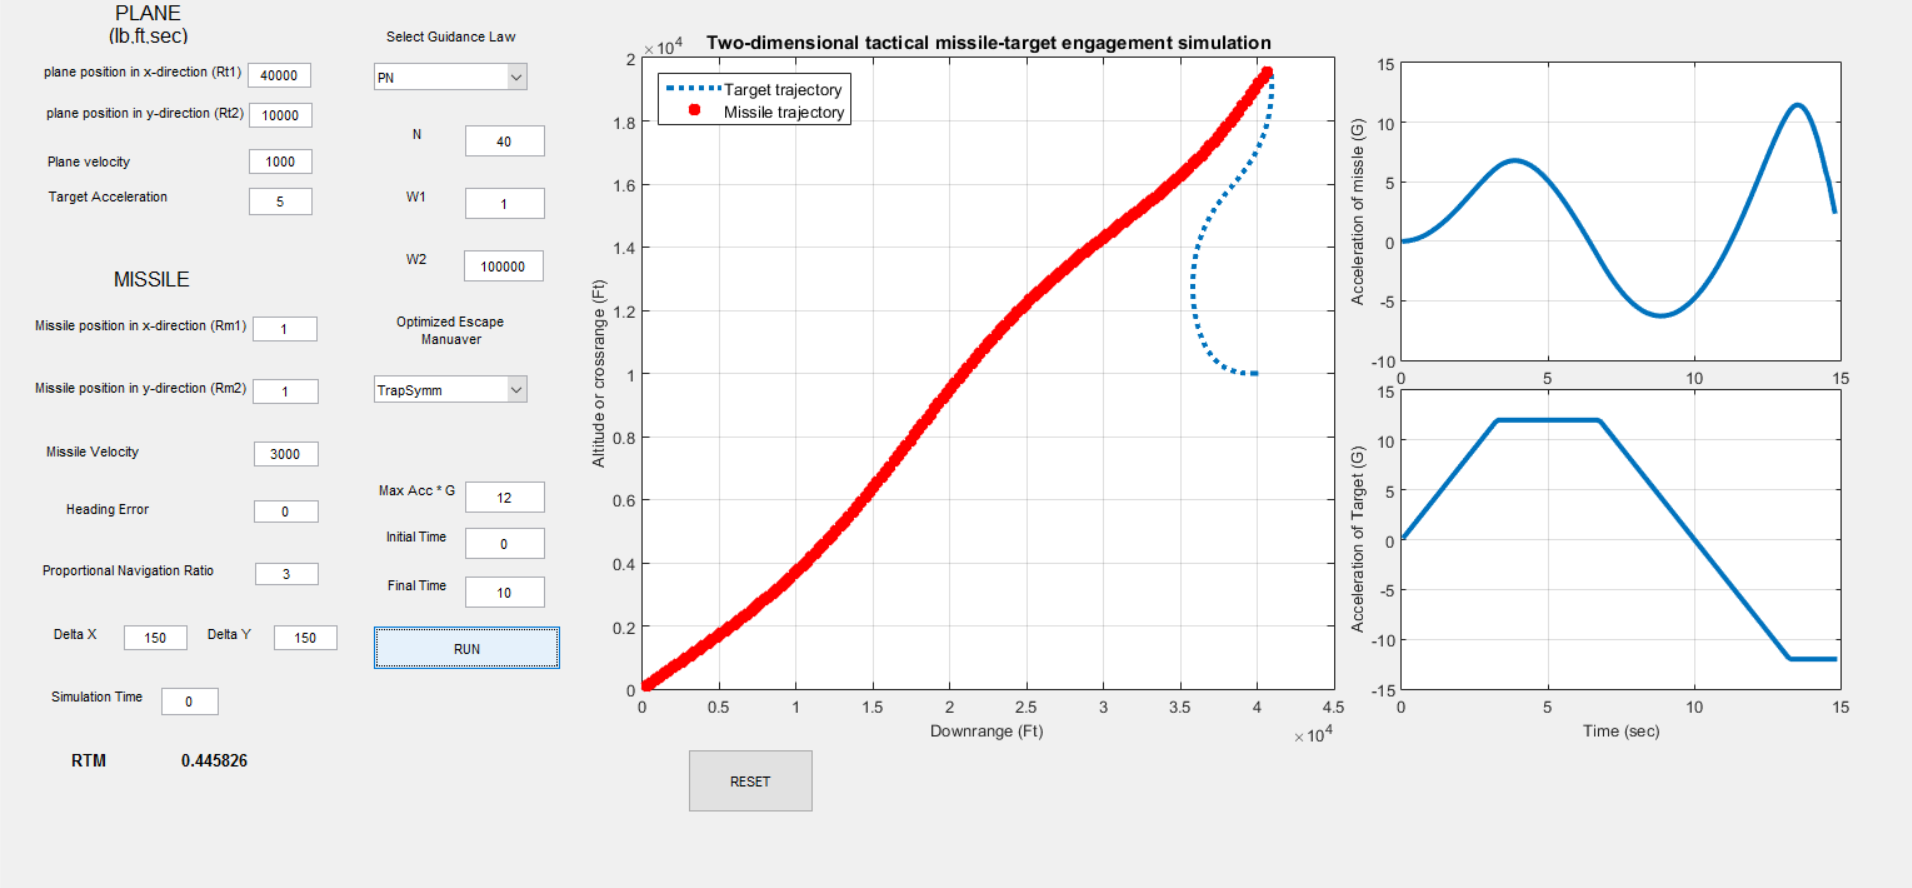
\includegraphics[scale = 0.4]{fig/guiPN.PNG}
	\caption{Guidance Toolbox options when PN selected}
	\label{Guidance Toolbox PN}
\end{figure}
  

%=============================================================================================
%=============================================================================================

\section{Genetic Algorithm Solution [using simulink]}


In this subsection we will use the power of blocks in Simulink to solve the differential equations in section \ref{PNeqations} in an easy way (Fig. \ref{PN eq}). We will make these equations as a main block (Fig. \ref{PN main block}) and as we change the inputs, we get the same results. The advantage of using simulink is to use the main block with an alternative optimization technique (like genetic algorithms) and we will simulate two cases, polynomial and trapezoidal. Now let us have a brief introduction to the genetic algorithm technique.

\subsection{Introduction to Genetic Algorithm technique}
Genetic algorithm is a \textit{stochastic population-based} search method. Genetic Algorithms (GAs) are   search algorithms based on the mechanics of the natural selection process (biological evolution).  The most basic concept is that the strong tend to adapt and survive while the weak tend to die out. That is, optimization is based on evolution, and the "Survival of the fittest" concept.
GAs have the ability to create an initial population of feasible solutions, and then recombine them in a way to guide their search to only the most promising areas of the state space.   
Each feasible solution is encoded as a chromosome (string) also called a genotype, and each chromosome is given a measure of fitness via a fitness (evaluation or objective) function. 

\begin{itemize}
	\item The fitness of a chromosome determines its ability to survive and produce offspring.
	\item A finite population of chromosomes is maintained.
	\item GAs  use  probabilistic  rules  to  evolve  a  population from  one  generation to the next.  The generations of the new solutions are developed by genetic recombination operators:
	\begin{itemize}
		\item Biased Reproduction: selecting the fittest to reproduce.
		\item Crossover: combining parent chromosomes to produce children chromosomes.
		\item Mutation: altering some genes in a chromosome.
	\end{itemize}
\end{itemize}

\subsubsection*{Most Important Parameters in GAs:}
\begin{itemize}
	\item Population Size
	\item Evaluation Function
	\item Crossover Method
	\item Mutation Rate
\end{itemize}

\subsubsection*{Use Genetic Algorithms:}
\begin{itemize}
	\item When facing a problem of local minima.
	\item When a good fitness function is available.
	\item When a near-optimal, but not optimal solution is acceptable.
	\item When the state-space is too large for other methods.
\end{itemize}

\subsection{COMPONENTS OF GENETIC ALGORITHMS}
\subsubsection*{Representation (definition of individuals):}
Objects forming possible solution within original problem context are called phenotypes, their encoding, the individuals within the GA, are called genotypes.
The representation step specifies the mapping from the phenotypes onto a set of genotypes.
Candidate solution, phenotype and individual are used to denote points of the space of possible solutions. This space is called phenotype space.
Chromosome, and individual can be used for points in the genotye space.
Elements of a chromosome are called genes. A value of a gene is called an allele.
The GA works with a coding of the parameter rather than the actual parameter. Depending  on the particular  problem,  the  coding  may  be  Boolean-valued,  integer-valued,  real-valued,   complex-valued, vector-valued,  symbolic  valued,  or multiple-valued.

\subsubsection*{Evaluation function:}
This is just the cost or the objective function which represent what we want to maximize. For minimization problem use the reciprocal (i.e. 1/f).

\subsubsection*{Population:}
The role of the population is to hold possible solutions. A population is a multiset of genotypes. In GA, the population size is (almost always) constant. The bigger the size, the better the final solution, and the larger the execution time.

\subsubsection*{Parent Selection Mechanism:}
The role of parent selection (mating selection) is to distinguish among individuals based on their quality to allow the better individuals to become parents of the next generation.
Parent selection is probabilistic. Thus, high quality individuals get a higher chance to become parents than those with low quality. Nevertheless, low quality individuals are often given a small, but positive chance; otherwise the whole search could become too greedy and get stuck in a local optimum.

\subsubsection*{Variation Operators:}
The role of variation operators is to create new individuals from old ones. Variation operators form the implementation of the elementary steps with the search space.

\subsubsection*{Mutation Operator:}
A unary variation operator is called \textit{mutation}. It is applied to one genotype and delivers a modified mutant, the child or \textit{offspring} of it.
In general, mutation is supposed to cause a random unbiased change. 

\subsubsection*{Crossover Operator:}
A binary variation operator is called recombination or crossover. This operator merges information from two parent genotypes into one or two offspring genotypes.
Similarly to mutation, crossover is a stochastic operator: the choice of what parts of each parent are combined, and the way these parts are combined, depend on random drawings.
The principle behind crossover is simple: by mating two individuals with different but desirable features, we can produce an offspring which combines both of those features.

\subsubsection*{Survivor Selection Mechanism:}
The role of survivor selection is to distinguish among individuals based on their quality. In GA, the population size is (almost always) constant, thus a choice has to be made on which individuals will be allowed in the next generation. This decision is based on their fitness values, favoring those with higher quality.
As opposed to parent selection which is stochastic, survivor selection is often deterministic, for instance, ranking the unified multiset of parents and offspring and selecting the top segment (fitness biased), or selection only from the offspring (age-biased).



\begin{landscape}
	\begin{figure}[H]
		\centering
		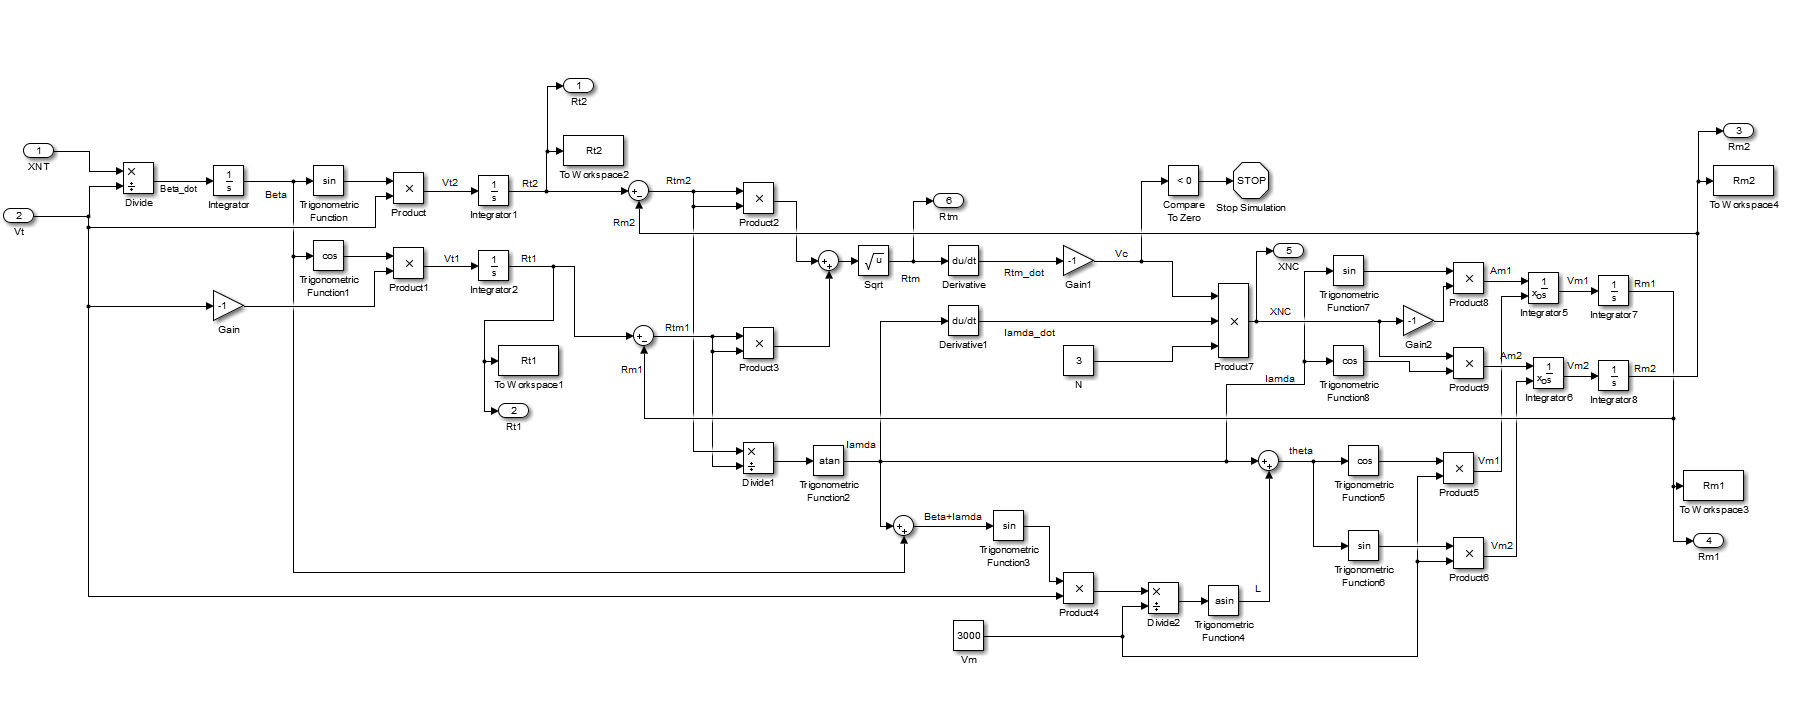
\includegraphics[scale = 0.70]{fig/PNeq.PNG}
		\caption{The Simulink model for proportional navigation equations in sec \ref{PNeqations}}
		\label{PN eq}
	\end{figure}
\end{landscape}


\begin{figure}[H]
	\centering
	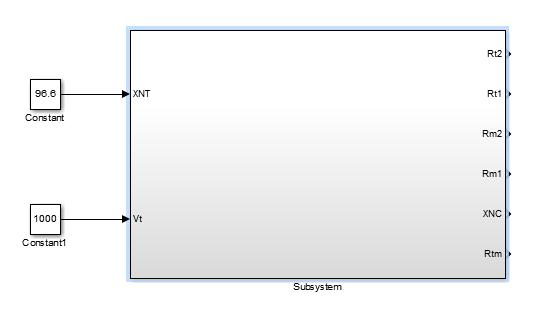
\includegraphics[scale = 0.75]{fig/PNmainBlock.PNG}
	\caption{The Simulink main block for solving proportional navigation equations in sec \ref{PNeqations}}
	\label{PN main block}
\end{figure}


%We will use the main block we have created with the genetic algorithm toolbox in MATLAB in the same manner we have done, let the target maneuver ba a polynomial with unknown coefficients, then it is required to find the values of these coefficients using genetic algorithm to maximize miss distance and missile acceleration.
%=======================================================

\subsection{Results}
We will use the main block we have created with the genetic algorithm toolbox in MATLAB in the same manner we have done, let the target maneuver unknown, then it is required to find it using genetic algorithm to maximize miss distance and missile acceleration. We have two cases of the target maneuver:

\subsubsection{Polynomial Target Maneuver}
let the target maneuver ba a polynomial with unknown coefficients, then it is required to find the values of these coefficients using genetic algorithm toolbox in Matlab (Fig. \ref{GA toolbox poly}) to maximize miss distance and missile acceleration. The result for the best fitness values are in Fig.\ref{GA poly F}. The optimized target acceleration and trajectory simulation are in figures \ref{GA poly XNT} and \ref{GA poly trajectory}. 

\begin{figure}[H]
	\centering
	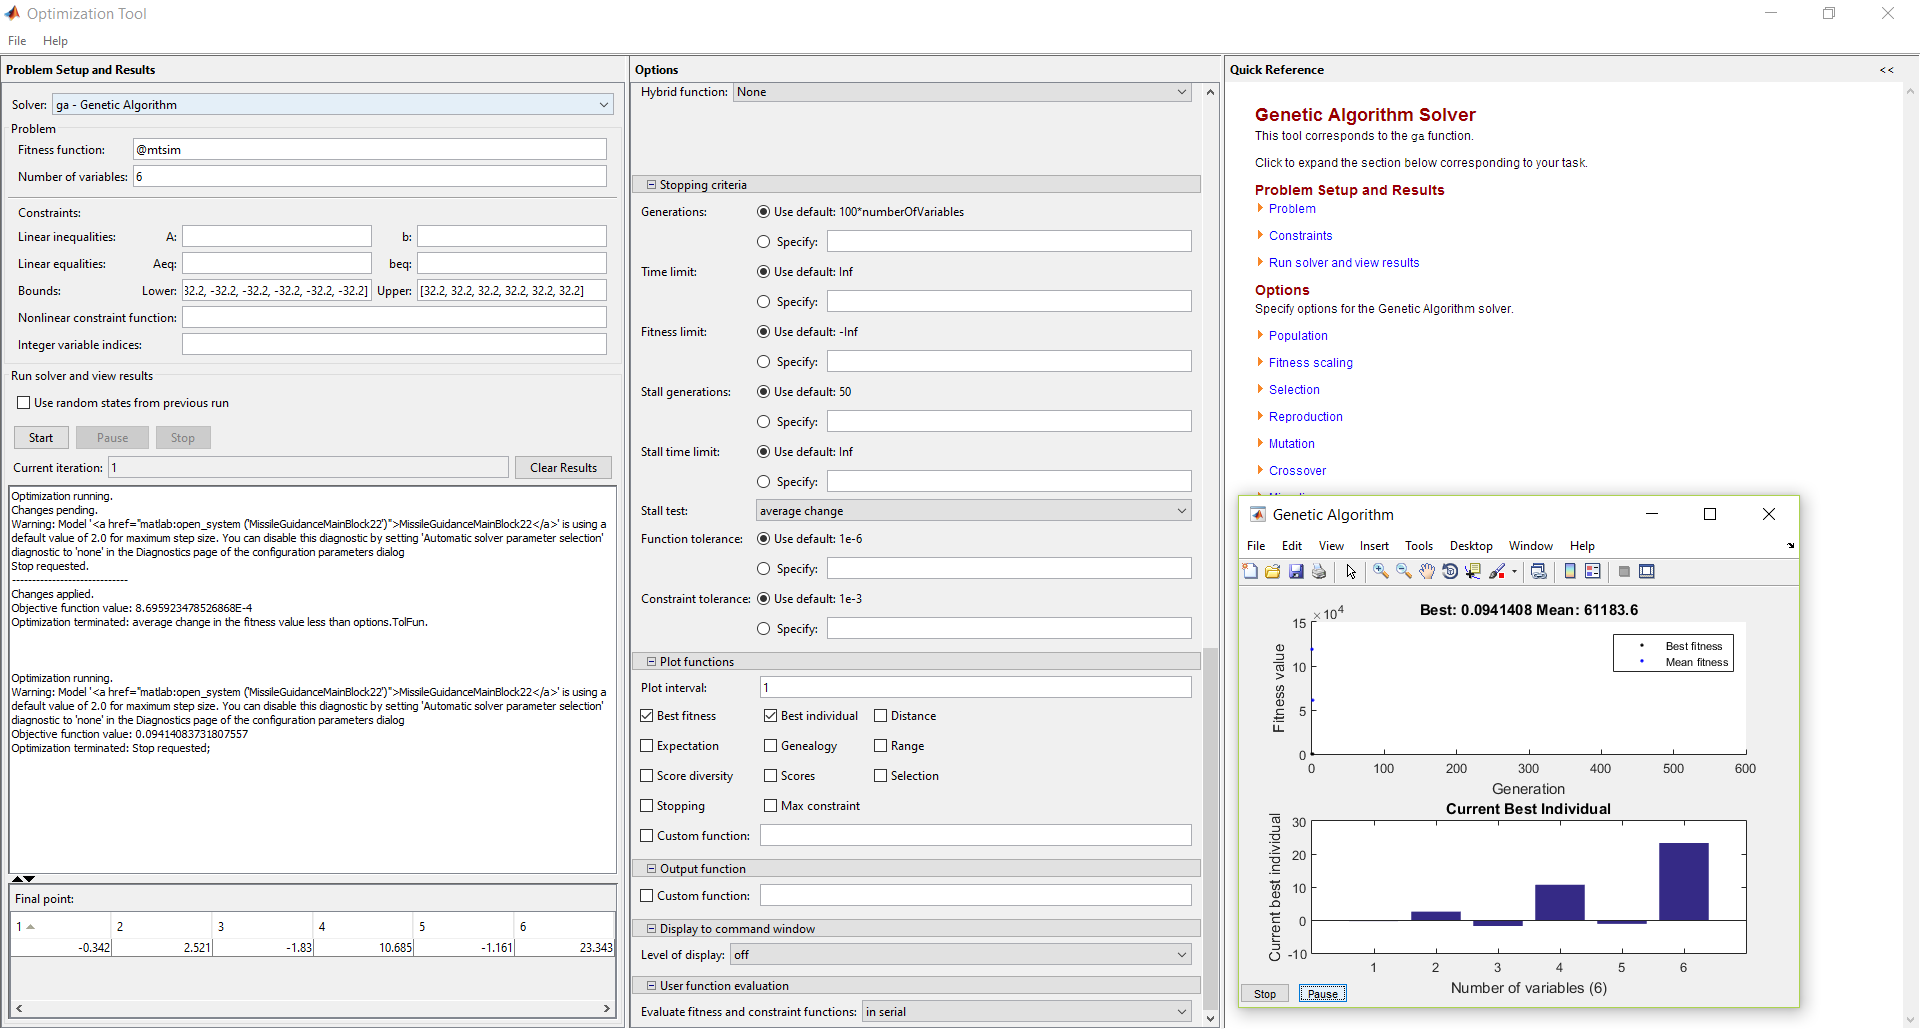
\includegraphics[scale = 0.4]{fig/GApoly.PNG}
	\caption{Genetic Algorithm Toolbox in Matlab.}
	\label{GA toolbox poly}
\end{figure}

\begin{figure}[H]
	\centering
	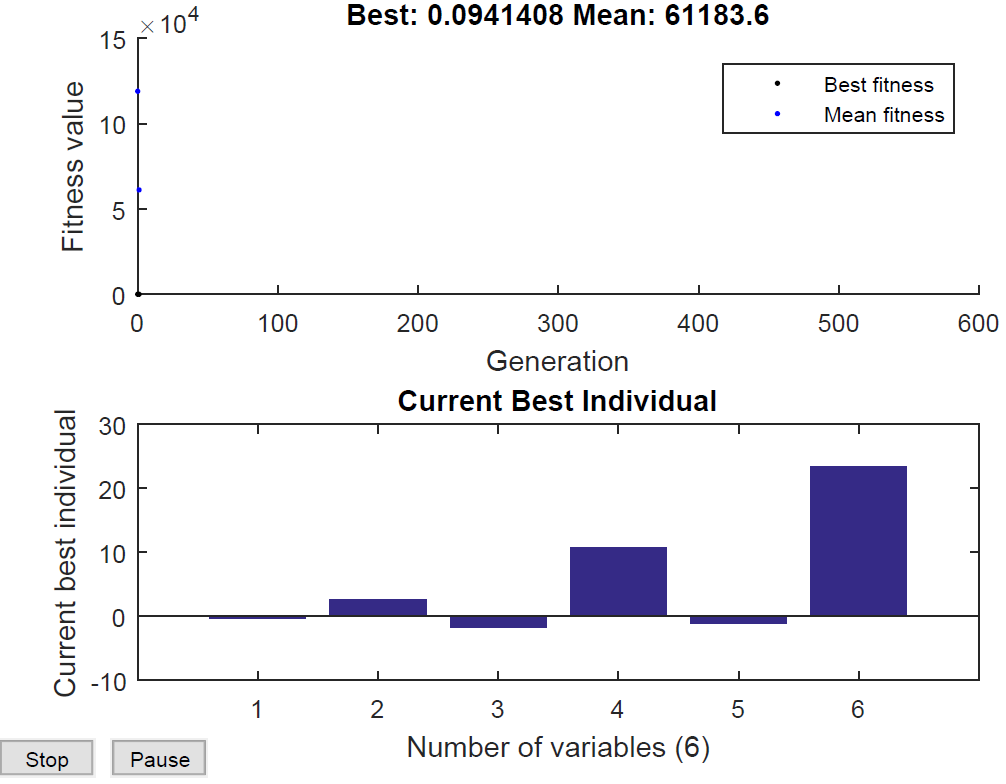
\includegraphics[scale = 0.4]{fig/GApolyF.PNG}
	\caption{Best fitness values}
	\label{GA poly F}
\end{figure}

\begin{figure}[H]
	\centering
	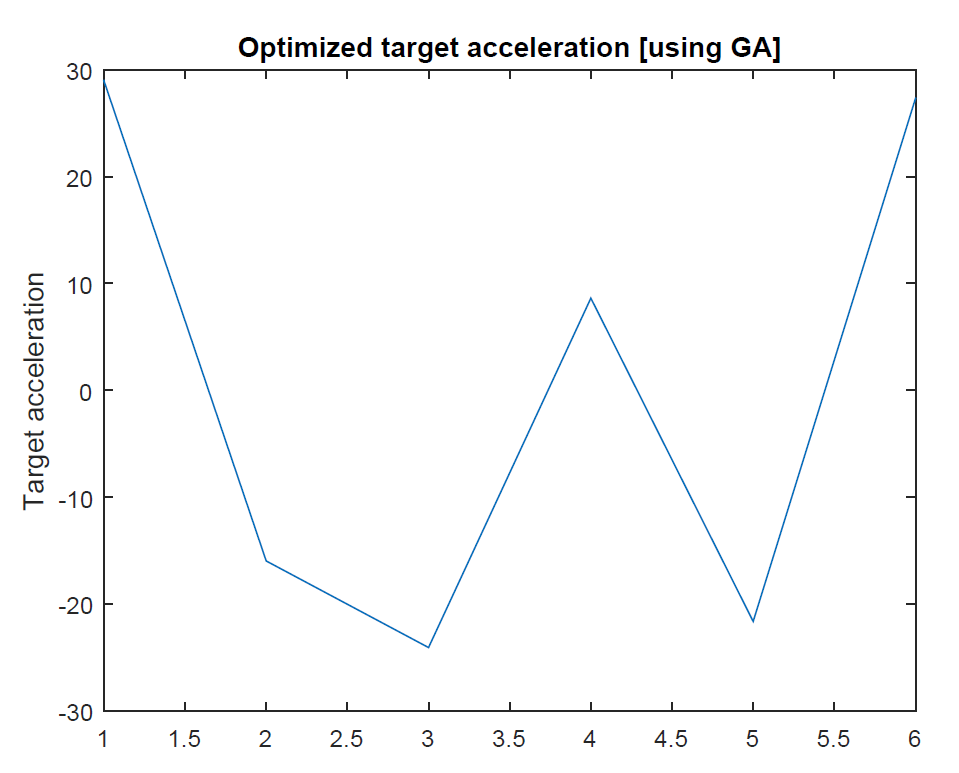
\includegraphics[scale = 0.4]{fig/GApolyXNT.PNG}
	\caption{Optimized target acceleration using GA.}
	\label{GA poly XNT}
\end{figure}


\begin{figure}[H]
	\centering
	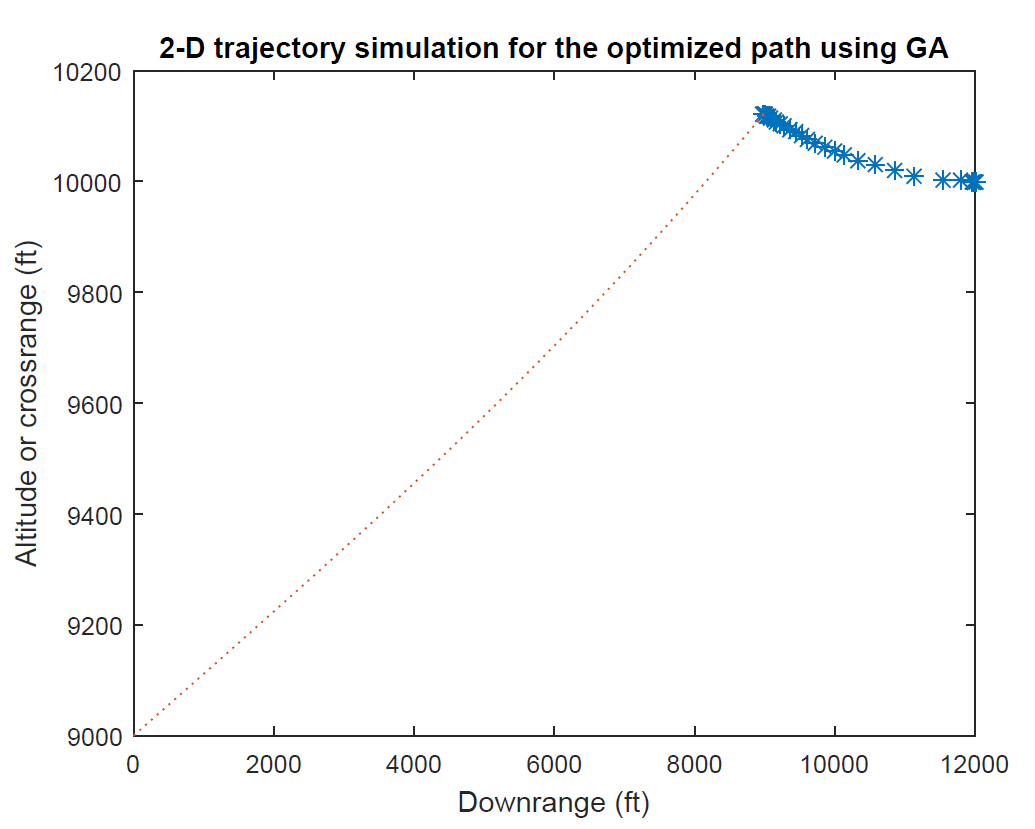
\includegraphics[scale = 0.4]{fig/polyTrajectory.PNG}
	\caption{Optimized trajectory using GA.}
	\label{GA poly trajectory}
\end{figure}

% ===================================================

